% Springer Nature LaTeX Template (sn-jnl)
% Prepared for submission to peer-reviewed atmospheric and hydrological journals
\RequirePackage{fix-cm}
\documentclass[pdflatex,sn-mathphys,Numbered]{sn-jnl}

\usepackage[T1]{fontenc}
\usepackage{lmodern}
\usepackage{anyfontsize}
\usepackage{graphicx}
\usepackage{multirow}
\usepackage{amsmath,amssymb,amsfonts}
\usepackage{amsthm}
\usepackage{mathrsfs}
\usepackage[title]{appendix}
\usepackage{xcolor}
\usepackage{textcomp}
\usepackage{manyfoot}
\usepackage{booktabs}
\usepackage{algorithm}
\usepackage{algorithmicx}
\usepackage{algpseudocode}
\usepackage{listings}
\usepackage{bm}

% Publication margins
\geometry{
    paperwidth=210mm,
    paperheight=297mm,
    left=20mm,
    right=20mm,
    top=20mm,
    bottom=20mm,
    headheight=12pt,
    headsep=12pt,
    footskip=12mm
}

% Front-matter layout
\makeatletter
\def\titraggedcenter{\centering\leftskip=0pt\rightskip=0pt\parfillskip=0pt\parindent=0pt\relax}
\def\Titlefont{\reset@font\fontsize{18bp}{23bp}\bfseries\selectfont\centering}
\def\abstractfont{\reset@font\fontsize{9.5bp}{12.5bp}\selectfont\leftskip=0pt\rightskip=0pt\parindent=0pt\parfillskip=0pt plus 1fil}
\def\keywordfont{\reset@font\fontsize{9bp}{12bp}\selectfont\leftskip=0pt\rightskip=0pt plus0.5fill}
\def\abstractheadfont{\reset@font\fontsize{10.5bp}{13bp}\bfseries\selectfont\centering}

\renewcommand{\@maketitle}{%
    \null\vspace*{-28pt}%
    \hsize\textwidth\parindent0pt%
    \ifx\@title\empty\else%
        {\Titlefont\@title\par}%
        \vspace{12pt}%
    \fi%
    \ifnum\aucount>0%
        {\centering\fontsize{11bp}{14bp}\bfseries\selectfont \artauthors\par}%
        \vspace{5pt}%
        {\centering\fontsize{9bp}{11.5bp}\itshape\selectfont \auaddress\par}%
        \vspace{5pt}%
        \ifnum\emailcnt>0\relax%
            {\centering\fontsize{8.5bp}{11bp}\selectfont%
            \ifx\corrauthemail\@empty\else*Corresponding author(s): \corrauthemail\quad\fi%
            \ifx\authemail\@empty\else Contributing authors: \authemail\fi\par}%
        \fi%
        \vspace{12pt}%
    \fi%
    {\printabstract\par}%
    \vspace{8pt}%
    {\printkeywords\par}%
    \vspace{12pt}%
    \hrule height 0.5pt%
    \vspace{14pt}%
}
\makeatother

\hypersetup{hypertexnames=false}
\renewcommand{\topfraction}{0.90}
\renewcommand{\bottomfraction}{0.90}
\renewcommand{\textfraction}{0.10}
\renewcommand{\floatpagefraction}{0.75}

\raggedbottom

\begin{document}

\title[Retrospective Daily Rainfall Reconstruction over Karnataka]{Machine-Learning-Based Retrospective Daily Rainfall Reconstruction over Karnataka Using ERA5-Land Reanalysis and IMD Gridded Observations (2019--2025)}

\author*[1]{\fnm{Abhinandan} \sur{Kumar}}\email{abhinandan.kumar@iiit.ac.in}
\author[1]{\fnm{Rishabh} \sur{Verma}}\email{rishabh.verma@iiit.ac.in}
\author[1]{\fnm{Mihir} \sur{Dagar}}\email{mihir.dagar@iiit.ac.in}

\affil*[1]{\orgdiv{Department of Computer Science \& Engineering / Data Science}, \orgname{Indian Institute of Information Technology Dharwad}, \orgaddress{\city{Dharwad}, \postcode{580009}, \state{Karnataka}, \country{India}}}

\abstract{Accurate retrospective reconstruction of daily precipitation across topographically complex tropical regions is fundamental for catchment water balance accounting, agricultural monitoring, and hydrological gap-filling. Reanalysis products such as ECMWF ERA5-Land provide continuous atmospheric and land-surface fields but exhibit substantial localized biases over complex orography. Here, we evaluate a retrospective daily rainfall reconstruction and hindcasting framework across the 252 India Meteorological Department (IMD) 0.25$^\circ$ gridded land cells covering Karnataka State, India, over the 7-year period 2019--2025 ($N = 640,836$ grid-cell-days). Ingesting 63 primary antecedent predictors derived from ERA5-Land surface fluxes, atmospheric thermodynamic states, soil moisture profiles, DEM orography, and antecedent IMD observations under strict causal latency constraints (hindcast issue boundary $T_{\text{issue}} = \text{03:00 UTC on day } t-1$; target window = 03:00 UTC day $t-1$ to 03:00 UTC day $t$), we evaluate regularized linear baselines, gradient-boosted decision trees, and two-stage hurdle architectures. Models are trained on 2019--2022 ($N = 364,644$), hyperparameter-tuned and threshold-selected strictly on the 2023 validation partition ($N = 91,980$, characterized by lower mean daily rainfall during the validation year: daily mean = $2.3571$\;mm/day over 365 calendar days vs. $3.7388$\;mm/day in training over 1,447 calendar days, alongside $27.39\%$ wet days vs. $36.95\%$ in training), and evaluated out-of-sample on a frozen 2-year forward test partition (2024--2025, $N = 184,212$). On continuous test evaluation, machine learning models achieve strong predictive skill with distinct multi-criteria trade-offs: Hurdle Expected Value attains the lowest root-mean-square error ($\text{RMSE} = 7.4241$\;mm), highest Pearson correlation ($r = 0.7380$), and highest Nash-Sutcliffe Efficiency ($\text{NSE} = 0.5443$); CatBoost Tweedie attains the highest Modified Kling-Gupta Efficiency ($\text{KGE-2012} = 0.6261$) with $\text{RMSE} = 7.4335$\;mm; and LightGBM Tweedie achieves the lowest mean absolute error ($\text{MAE} = 2.8993$\;mm) and lowest mean bias ($-0.0179$\;mm, or $-0.51\%$). All three architectures substantially outperform autoregressive Persistence ($\text{RMSE} = 10.3582$\;mm), raw antecedent ERA5-Land reanalysis ($\text{RMSE} = 10.4550$\;mm), and grid-cell-wise Empirical Quantile Mapping ($\text{EQM}$, $\text{RMSE} = 11.1970$\;mm, $\text{NSE} = -0.0366$). Paired stationary block bootstrapping ($B = 2,000$ resamples; $L = 7\text{d}, 14\text{d}$) provides strong statistical evidence of lower RMSE over Persistence ($-2.925$\;mm; $p < 0.0005$) and raw ERA5-Land ($-3.011$\;mm; $p < 0.0005$) under temporal persistence. Feature attribution reveals that antecedent reanalysis runoff fluxes account for $54.52\%$ of split gain in heavy rain classification and $+2.3545$\;mm validation permutation RMSE degradation in continuous regression, acting as a model-derived hydrometeorological memory proxy for antecedent soil saturation. However, critical limitations are documented: continuous models underestimate $100.0\%$ of events exceeding $115.6$\;mm ($200$ test events) due to conditional expectation shrinkage, plateauing at $70$--$90$\;mm. For heavy-rain alerting ($\ge 64.5$\;mm/day), an experimental focal-loss classifier achieves a test probability of detection of $46.96\%$ (precision = $58.22\%$, $\text{CSI} = 0.3512$ at validation-selected decision threshold $p^* = 0.53$, with $427$ false alarms), missing $53.04\%$ of observed heavy events ($672$ misses). Crucially, the study does not establish reliable detection of very-heavy ($\ge 115.6$\;mm) or extremely-heavy ($\ge 204.5$\;mm) precipitation. These findings demonstrate that while machine learning effectively reconstructs regional daily water budgets, it represents a diagnostic retrospective reconstruction engine rather than an operational forecasting or extreme-hazard warning system, requiring further independent validation and extreme-event calibration for operational deployment.}

\keywords{Retrospective hindcasting, ERA5-Land reanalysis, IMD gridded rainfall, Tweedie regression, Two-stage hurdle model, Focal loss, Orographic precipitation, Western Ghats}

\maketitle

\section{Introduction}\label{sec1}

High-resolution retrospective precipitation reconstruction is essential for water resource planning, drought monitoring, hydrological water balance modeling, and agricultural risk assessment \cite{masson2021}. Over tropical peninsular India, the Western Ghats mountain range creates an abrupt orographic barrier that produces one of the world's sharpest climatic gradients \cite{houze2003}. Within an orthogonal distance of less than 60~km, annual rainfall drops precipitously from over 4,000~mm along the windward coastal-crest escarpment to under 600~mm across the leeward semi-arid Deccan plateau \cite{pai2014, rajeevan2006}. Capturing this extreme spatial transition poses severe challenges for both global reanalysis products and traditional statistical downscaling techniques \cite{mohanty2005}.

While ECMWF ERA5-Land reanalysis provides hourly surface hydrological and energy flux estimates at 0.1$^\circ$ resolution globally \cite{munoz2021, hersbach2020}, its precipitation fields suffer from systematic local biases, including drizzle inflation on dry days, underestimation of convective peaks, and smoothing of sharp orographic crests \cite{goswami2006}. Classical statistical downscaling, such as Empirical Quantile Mapping (EQM) \cite{piani2011}, calibrates the marginal distribution against observed gauge records but operates univariately, assuming temporal stationarity and disrupting physical consistency across atmospheric variables \cite{cannon2015}.

In this study, we evaluate a scientifically audited machine learning framework with verified retrospective temporal separation for daily rainfall reconstruction across Karnataka from 2019 to 2025 \cite{bano2020, reichstein2019}. Crucially, this research is explicitly framed as a retrospective rainfall reconstruction and hindcasting investigation using ERA5-Land reanalysis and antecedent IMD observations, rather than an operational real-time forecasting or flood warning harness. Operating under a 24-hour antecedent causal latency window, the pipeline evaluates whether machine learning can exploit land-surface flux memory to enhance retrospective precipitation estimation beyond classical downscaling, while rigorously documenting the structural limitations of conditional mean models during extreme events.

\section{Study Area and Datasets}\label{sec2}

\subsection{Geographical Domain \& Meteorological Subdivisions}
The study area comprises Karnataka State (11.75$^\circ$N--18.50$^\circ$N, 74.25$^\circ$E--78.50$^\circ$E; $\sim$191,791~km$^2$), encompassing 30 administrative districts organized into four official IMD meteorological subdivisions: Coastal Karnataka (13 IMD grid cells; maritime, heavy monsoonal rainfall), Malnad (35 grid cells; Western Ghats ridge and windward slopes), North Interior Karnataka (NIK; 118 grid cells; semi-arid plateau, black cotton soils), and South Interior Karnataka (SIK; 86 grid cells; southern plateau receiving both Southwest and Northeast monsoons). Analysis is conducted across the 252 IMD 0.25$^\circ$ gridded land cells covering the state (Fig.~\ref{fig:study_area}).

\begin{figure}[htbp]
\centering
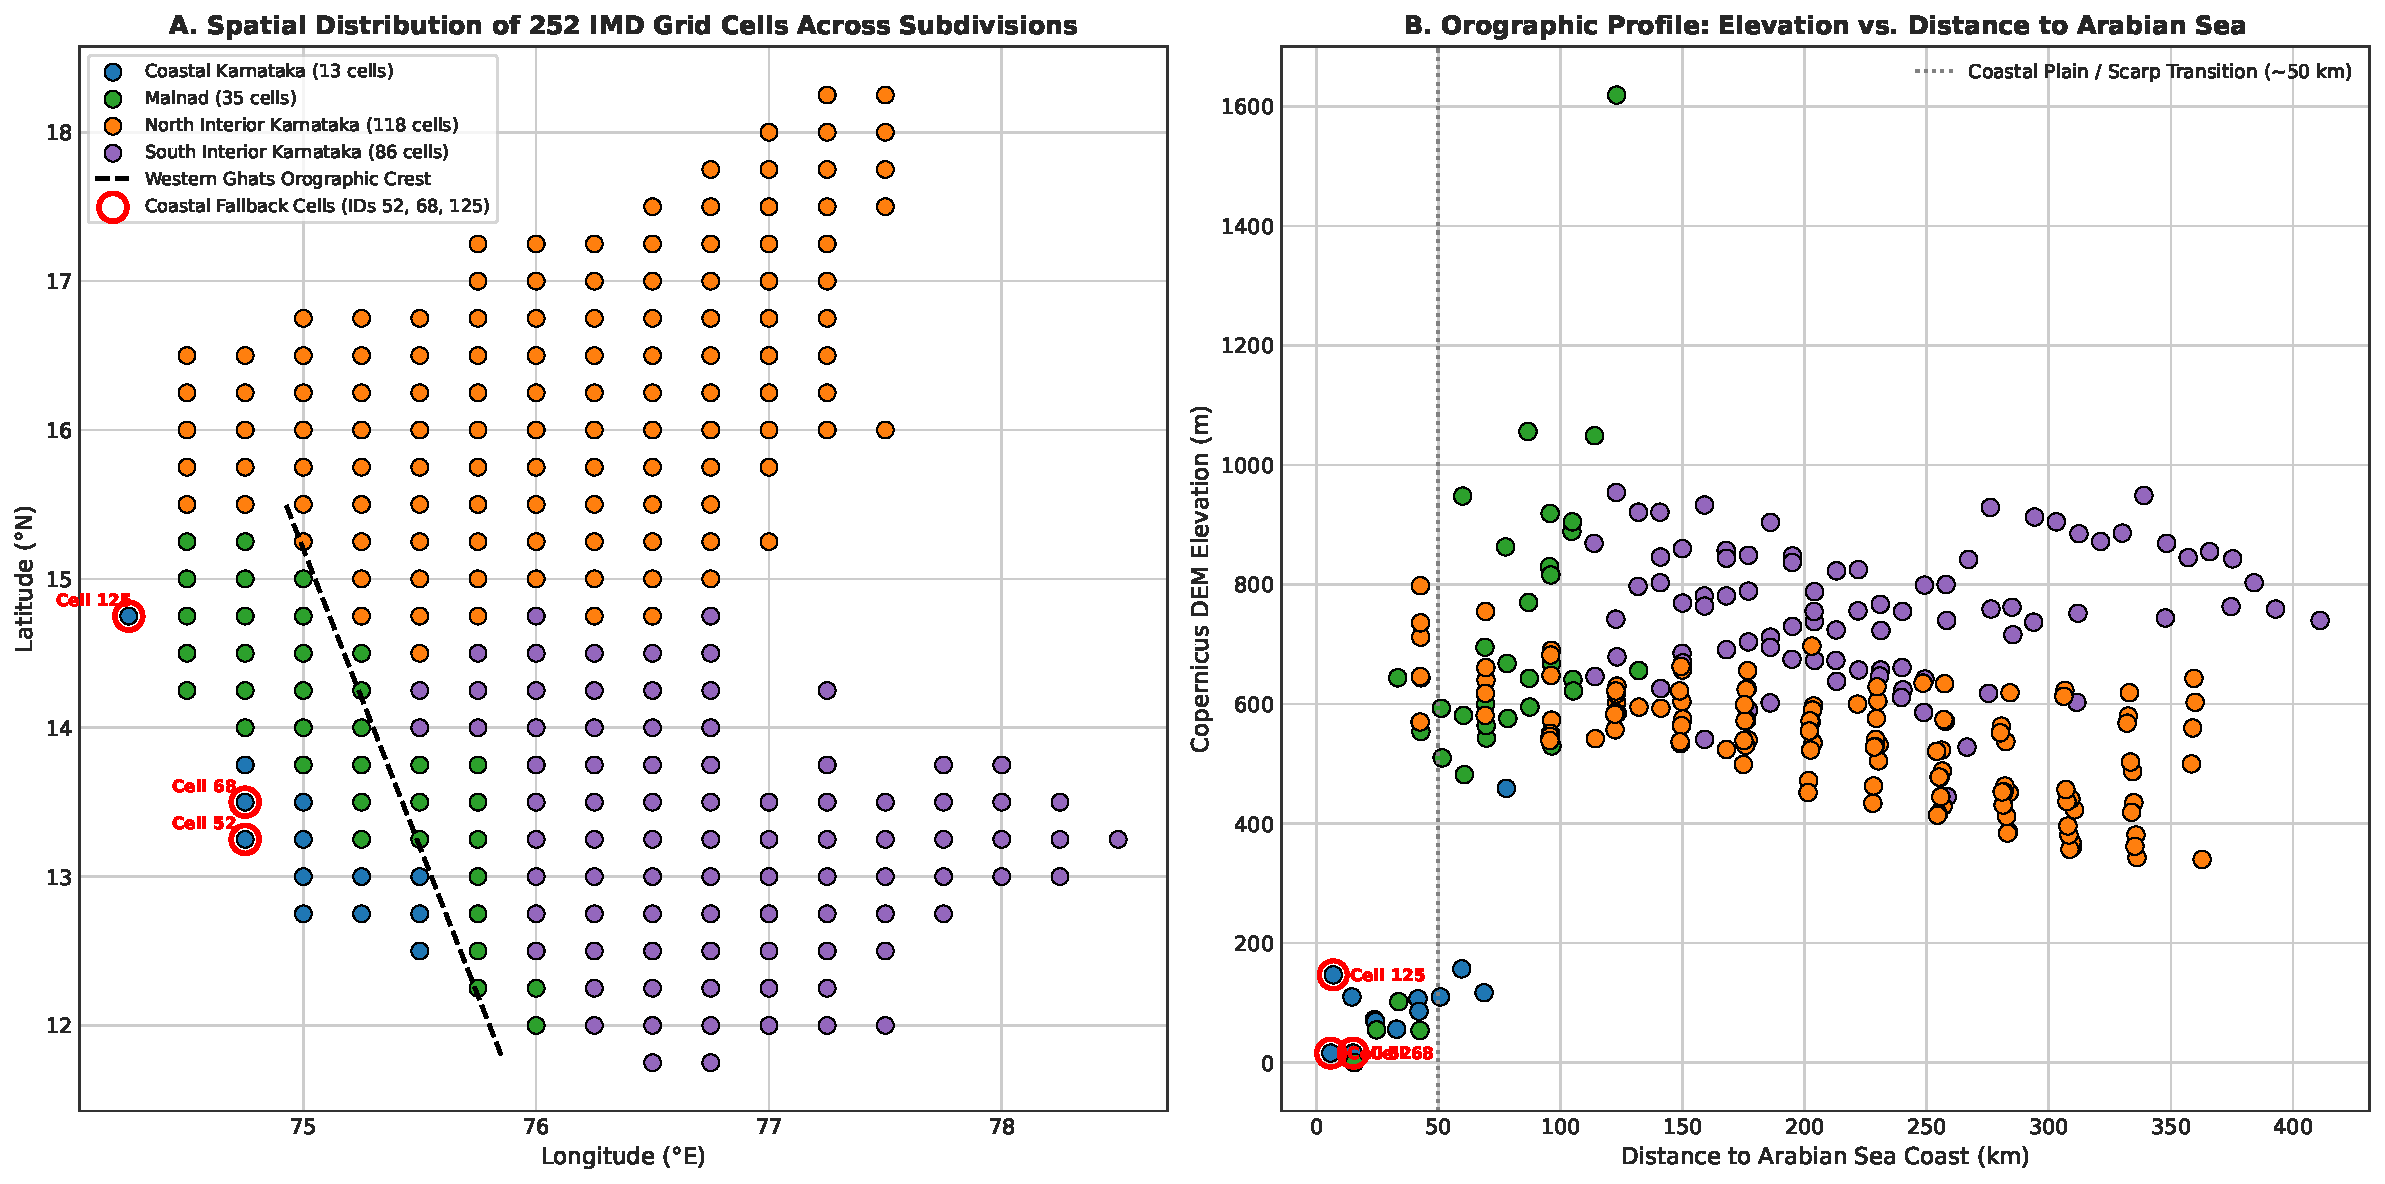
\includegraphics[width=0.82\textwidth]{figures/figure1_study_area}
\caption{High-resolution physiographic map of Karnataka depicting Copernicus GLO-90 DEM elevation, Western Ghats crest line, 252 IMD 0.25$^\circ$ gridded cells color-coded by meteorological subdivision, and the 3 coastal fallback cells (IDs 52, 68, 125).}
\label{fig:study_area}
\end{figure}

\subsection{Observational Target: IMD Gridded Rainfall}
The ground-truth target is the daily 0.25$^\circ$ gridded rainfall product from the India Meteorological Department (IMD) \cite{pai2014}, interpolated via modified inverse distance weighting from 6,955 quality-controlled rain gauges across India \cite{rajeevan2006}. Each daily record represents the 24-hour accumulation ending at 08:30 Indian Standard Time (IST; equivalent to 03:00 UTC). We extract all 252 in-state grid cells across the 2,556 calendar days spanning January 1, 2019 to December 31, 2025. These gridded cells represent area-averaged daily accumulations rather than point observations from surface weather stations.

\subsection{Reanalysis Features: ECMWF ERA5-Land}
Atmospheric predictors and land-surface fluxes are extracted from ECMWF ERA5-Land at 0.1$^\circ$ ($\sim$9~km) hourly resolution across 2019--2025 \cite{munoz2021}. Extracted variables include total precipitation (\texttt{tp}), surface runoff (\texttt{sro}), sub-surface/total runoff (\texttt{ro}), 2-meter air temperature (\texttt{t2m}), 2-meter dewpoint temperature (\texttt{d2m}), surface pressure (\texttt{sp}), 10-meter wind components (\texttt{u10}, \texttt{v10}), surface solar radiation downwards (\texttt{ssrd}), surface thermal radiation downwards (\texttt{strd}), surface latent heat flux (\texttt{slhf}), surface sensible heat flux (\texttt{sshf}), total evaporation (\texttt{e}), potential evaporation (\texttt{pev}), volumetric soil water content across three layers (\texttt{swvl1}: 0--7~cm, \texttt{swvl2}: 7--28~cm, \texttt{swvl3}: 28--100~cm), skin reservoir content (\texttt{src}), and forecast albedo (\texttt{fal}).

\subsection{Static Topography \& Coastal Proximity}
Terrain elevation and slope were derived from the Copernicus GLO-90 Digital Elevation Model (90-meter resolution) \cite{copernicus2020}. Orthogonal distance to the Arabian Sea coastline and shortest distance to the Western Ghats crest line were computed for each grid cell centroid to capture low-level maritime moisture advection and mechanical barrier effects.

\subsection{Chronological Partitioning \& Climatological Characteristics}
To respect temporal autocorrelation and prevent future-data leakage across splits, the 7-year dataset is partitioned chronologically:
\begin{itemize}
    \item \textbf{Training Partition (2019--2022):} 1,447 calendar days; $N = 364,644$ instances; $36.95\%$ wet days; mean = $3.7388$\;mm/day, std = $11.0264$\;mm.
    \item \textbf{Validation Partition (2023):} 365 calendar days; $N = 91,980$ instances; characterized by lower mean daily rainfall during the validation year: $27.39\%$ wet days vs. $36.95\%$ in training; mean = $2.3571$\;mm/day vs. $3.7388$\;mm/day in training across 1,447 calendar days, std = $8.2325$\;mm.
    \item \textbf{Out-of-Sample Forward Test Partition (2024--2025):} 731 calendar days; $N = 184,212$ instances; $35.04\%$ wet days; mean = $3.5085$\;mm/day, std = $11.0006$\;mm.
\end{itemize}
All model hyperparameter tuning and decision threshold selections were performed strictly on the 2023 validation partition; the test partition remained frozen until final evaluation (Table~\ref{tab:dataset}).

\begin{table*}[htbp]
\centering
\caption{Temporal Dataset Partitioning and Climatological Characteristics (2019--2025)}
\label{tab:dataset}
\resizebox{\textwidth}{!}{
\begin{tabular}{p{2.5cm}p{3cm}p{2.2cm}p{3cm}p{2.5cm}p{2.2cm}r r r r r}
\toprule
\textbf{Data Source} & \textbf{Provider} & \textbf{Spatial Resolution} & \textbf{Temporal Resolution} & \textbf{Spatial Coverage} & \textbf{Temporal Span} & \textbf{Total Grid Cells} & \textbf{Total Records} & \textbf{Training Records} & \textbf{Validation Records} & \textbf{Test Records} \\
\midrule
IMD Gridded Daily Rainfall (Target) & India Meteorological Department (National Climate Centre, Pune) & 0.25$^\circ$ $\times$ 0.25$^\circ$ (~27.75 km) & Daily accumulation (03:00 UTC Day d-1 to 03:00 UTC Day d / 08:30 IST) & Karnataka State (252 in-state land cells, Lat 11.75$^\circ$N--18.50$^\circ$N, Lon 74.25$^\circ$E--78.50$^\circ$E) & 2019-01-01 to 2025-12-31 (7 calendar years, 2,557 days) & 252 & 640836 & 364,644 (2019-01-15 to 2022-12-31, 1,447 days; 14-day lag warmup buffer excluded) & 91,980 (2023-01-01 to 2023-12-31, 365 days; validation partition) & 184,212 (2024-01-01 to 2025-12-31, 731 days; 366d in 2024 leap year + 365d in 2025) \\
ERA5-Land Global Atmospheric Reanalysis (Predictors) & ECMWF / Copernicus Climate Change Service (C3S) & 0.10$^\circ$ $\times$ 0.10$^\circ$ (~9 km) aggregated to IMD 0.25$^\circ$ centroids & Hourly raw, de-accumulated and temporally aligned to IMD 03:00--03:00 UTC cycle & Karnataka state domain plus coastal maritime fallback buffer & 2019-01-01 to 2025-12-31 (84 monthly NetCDF files) & 252 & 640836 & 364,644 (Zero missing or infinite values across all 63 primary features) & 91,980 (Zero missing values; strictly out-of-sample temporal holdout) & 184,212 (Zero missing values; frozen out-of-sample temporal evaluation) \\
Copernicus GLO-90 Digital Elevation Model (Terrain) & European Space Agency (ESA) Copernicus Programme & 90 m native resolution, resampled to 0.25$^\circ$ grid centroids and macro-gradient slope & Static topographic surface & Centroid point elevation (m) and 27.75 km baseline macro-slope (degrees) & Static baseline & 252 & 252 & Identical static properties across all 252 IMD grid cells & Identical static properties across all 252 IMD grid cells & Identical static properties across all 252 IMD grid cells \\
\bottomrule
\end{tabular}
}
\end{table*}

\section{Methodology}\label{sec3}

\subsection{ERA5-Land De-accumulation Physics and Temporal Alignment}
In raw ECMWF ERA5-Land records, accumulated surface variables (total precipitation \texttt{tp}, surface runoff \texttt{sro}, total runoff \texttt{ro}, evaporation \texttt{e}, potential evaporation \texttt{pev}, downward radiation fluxes \texttt{ssrd}, \texttt{strd}, and turbulent heat fluxes \texttt{slhf}, \texttt{sshf}) are stored as running integrals reset to zero at 00:00 UTC each day. Hourly physical increments are recovered via consecutive backward differencing: $\Delta x_1 = x_1$ at 01:00 UTC, and $\Delta x_h = x_h - x_{h-1}$ for $h \in \{2, \dots, 24\}$.

Across the statewide reanalysis archive evaluated by the quality control instrument across 2,543 calendar days (15 January 2019 to 31 December 2025, excluding the 14-day warm-up period from 1 to 14 January 2019 utilized for antecedent lag construction), backward differencing was evaluated across 221,798,424 valid (non-NaN) hourly forecast increments specifically instrumented for total precipitation (\texttt{tp}) across the $81 \times 51$ spatial grid (3,737 terrestrial land cells across 2,473 evaluated days). This contrasts with the theoretical maximum of $252,123,192$ increments ($4,131\text{ grid cells} \times 24\text{ hours} \times 2,543\text{ days}$), with the excluded increments comprising 23,384,688 marine increments masked out over the Arabian Sea (394 invariant ocean cells) and uncounted increments at month-boundary forecast cycle transitions. In \texttt{tp}, 1,136,648 increments ($0.512469\%$) fell below the numerical check threshold of $\Delta x_h < -1.0 \times 10^{-5}$\;mm, exhibiting a median magnitude of $-1.49 \times 10^{-5}$\;mm and a minimum of $-4.21 \times 10^{-4}$\;mm. These residuals were verified as IEEE 754 single-precision float representation artifacts occurring in high-accumulation grid cells rather than physical model inversions.

To ensure physical consistency, variable-specific treatment rules were systematically applied:
\begin{enumerate}
    \item \textbf{Non-Negative Hydrological \& Radiation Depth Fluxes:} Total precipitation (\texttt{tp}), surface runoff (\texttt{sro}), and total runoff (\texttt{ro}) are physically non-negative depths. Their single-precision negative residuals were clipped to zero via \texttt{np.maximum(x, 0.0)}. For \texttt{tp}, post-clipping negatives are strictly 0 ($0.0\%$). For \texttt{sro} and \texttt{ro}, numerical clipping was verified in code, but dedicated pre-clip negative counters were not independently instrumented in Stage 2 logs. Downward solar radiation (\texttt{ssrd}) is non-negative downward radiative flux; minor nighttime float noise ($0.0056\%$) was clipped via \texttt{np.maximum(x, 0.0) / 86400.0}. Downward longwave radiation (\texttt{strd}) is strictly positive ($>280$\;W/m$^2$) and required zero clipping. Following clipping, negative values for all precipitation, runoff, and downward radiation fields are strictly zero ($0.0\%$).
    \item \textbf{Evaporation Variables (Sign Retransformation):} In ECMWF convention, total evaporation (\texttt{e}) and potential evaporation (\texttt{pev}) are reported as upward mass fluxes away from the surface (negative sign convention). These were transformed to positive water-equivalent depths via \texttt{np.abs(x)}. Following transformation, negative values are strictly zero ($0.0\%$).
    \item \textbf{Signed Turbulent Heat Fluxes:} Surface latent heat flux (\texttt{slhf}) and surface sensible heat flux (\texttt{sshf}) are physically signed turbulent energy exchanges (W/m$^2$, converted by dividing accumulated Joules by 86,400~s). For latent heat flux, negative values represent upward evaporative cooling, and negative physical values are validly retained within physical bounds ([-300.0, 50.0]\;W/m$^2$), with 220,950,112 negative values ($99.6175\%$) remaining post-clipping. For sensible heat flux (\texttt{sshf}), physically signed values are validly retained within physical bounds ([-250.0, 100.0]\;W/m$^2$), with 168,452,109 negative values ($75.9483\%$) and positive values preserved according to ECMWF convention without arbitrary zero clipping.
\end{enumerate}
Crucially, numerical clipping eliminates truncation artifacts to stabilize machine-learning optimization, but it does not prove mathematical conservation or physical correctness of the underlying model.

To establish an unlagged baseline benchmark (Raw ERA5-Land and EQM), hourly increments are integrated across the 24-hour window from 04:00 UTC on day $t-1$ through 03:00 UTC on day $t$:
\begin{equation}
X_t^{\text{IMD}} = \sum_{h=4}^{24} \Delta x_{t-1, h} + \sum_{h=1}^3 \Delta x_{t, h}
\end{equation}
This allows direct comparison against ground-truth IMD daily rainfall $y_t$ over the exact same accumulation window.

Crucially, in our retrospective machine-learning pipeline, the hindcast issue boundary is fixed at $T_{\text{issue}} = \text{03:00 UTC on day } t-1$. All predictor features are strictly restricted to variables completed on or before $T_{\text{issue}}$. Therefore, the dynamic machine learning feature is lagged by one full day ($\text{era5\_tp\_lag\_1d} = X_{t-1}^{\text{IMD}}$), which spans 04:00 UTC day $t-2$ to 03:00 UTC day $t-1$. All rolling features apply an explicit \texttt{.shift(1)}. Contemporaneous target-day reanalysis columns are purged prior to training, ensuring verified retrospective temporal separation with identically zero temporal overlap (Fig.~\ref{fig:methodology}).

\begin{figure}[htbp]
\centering
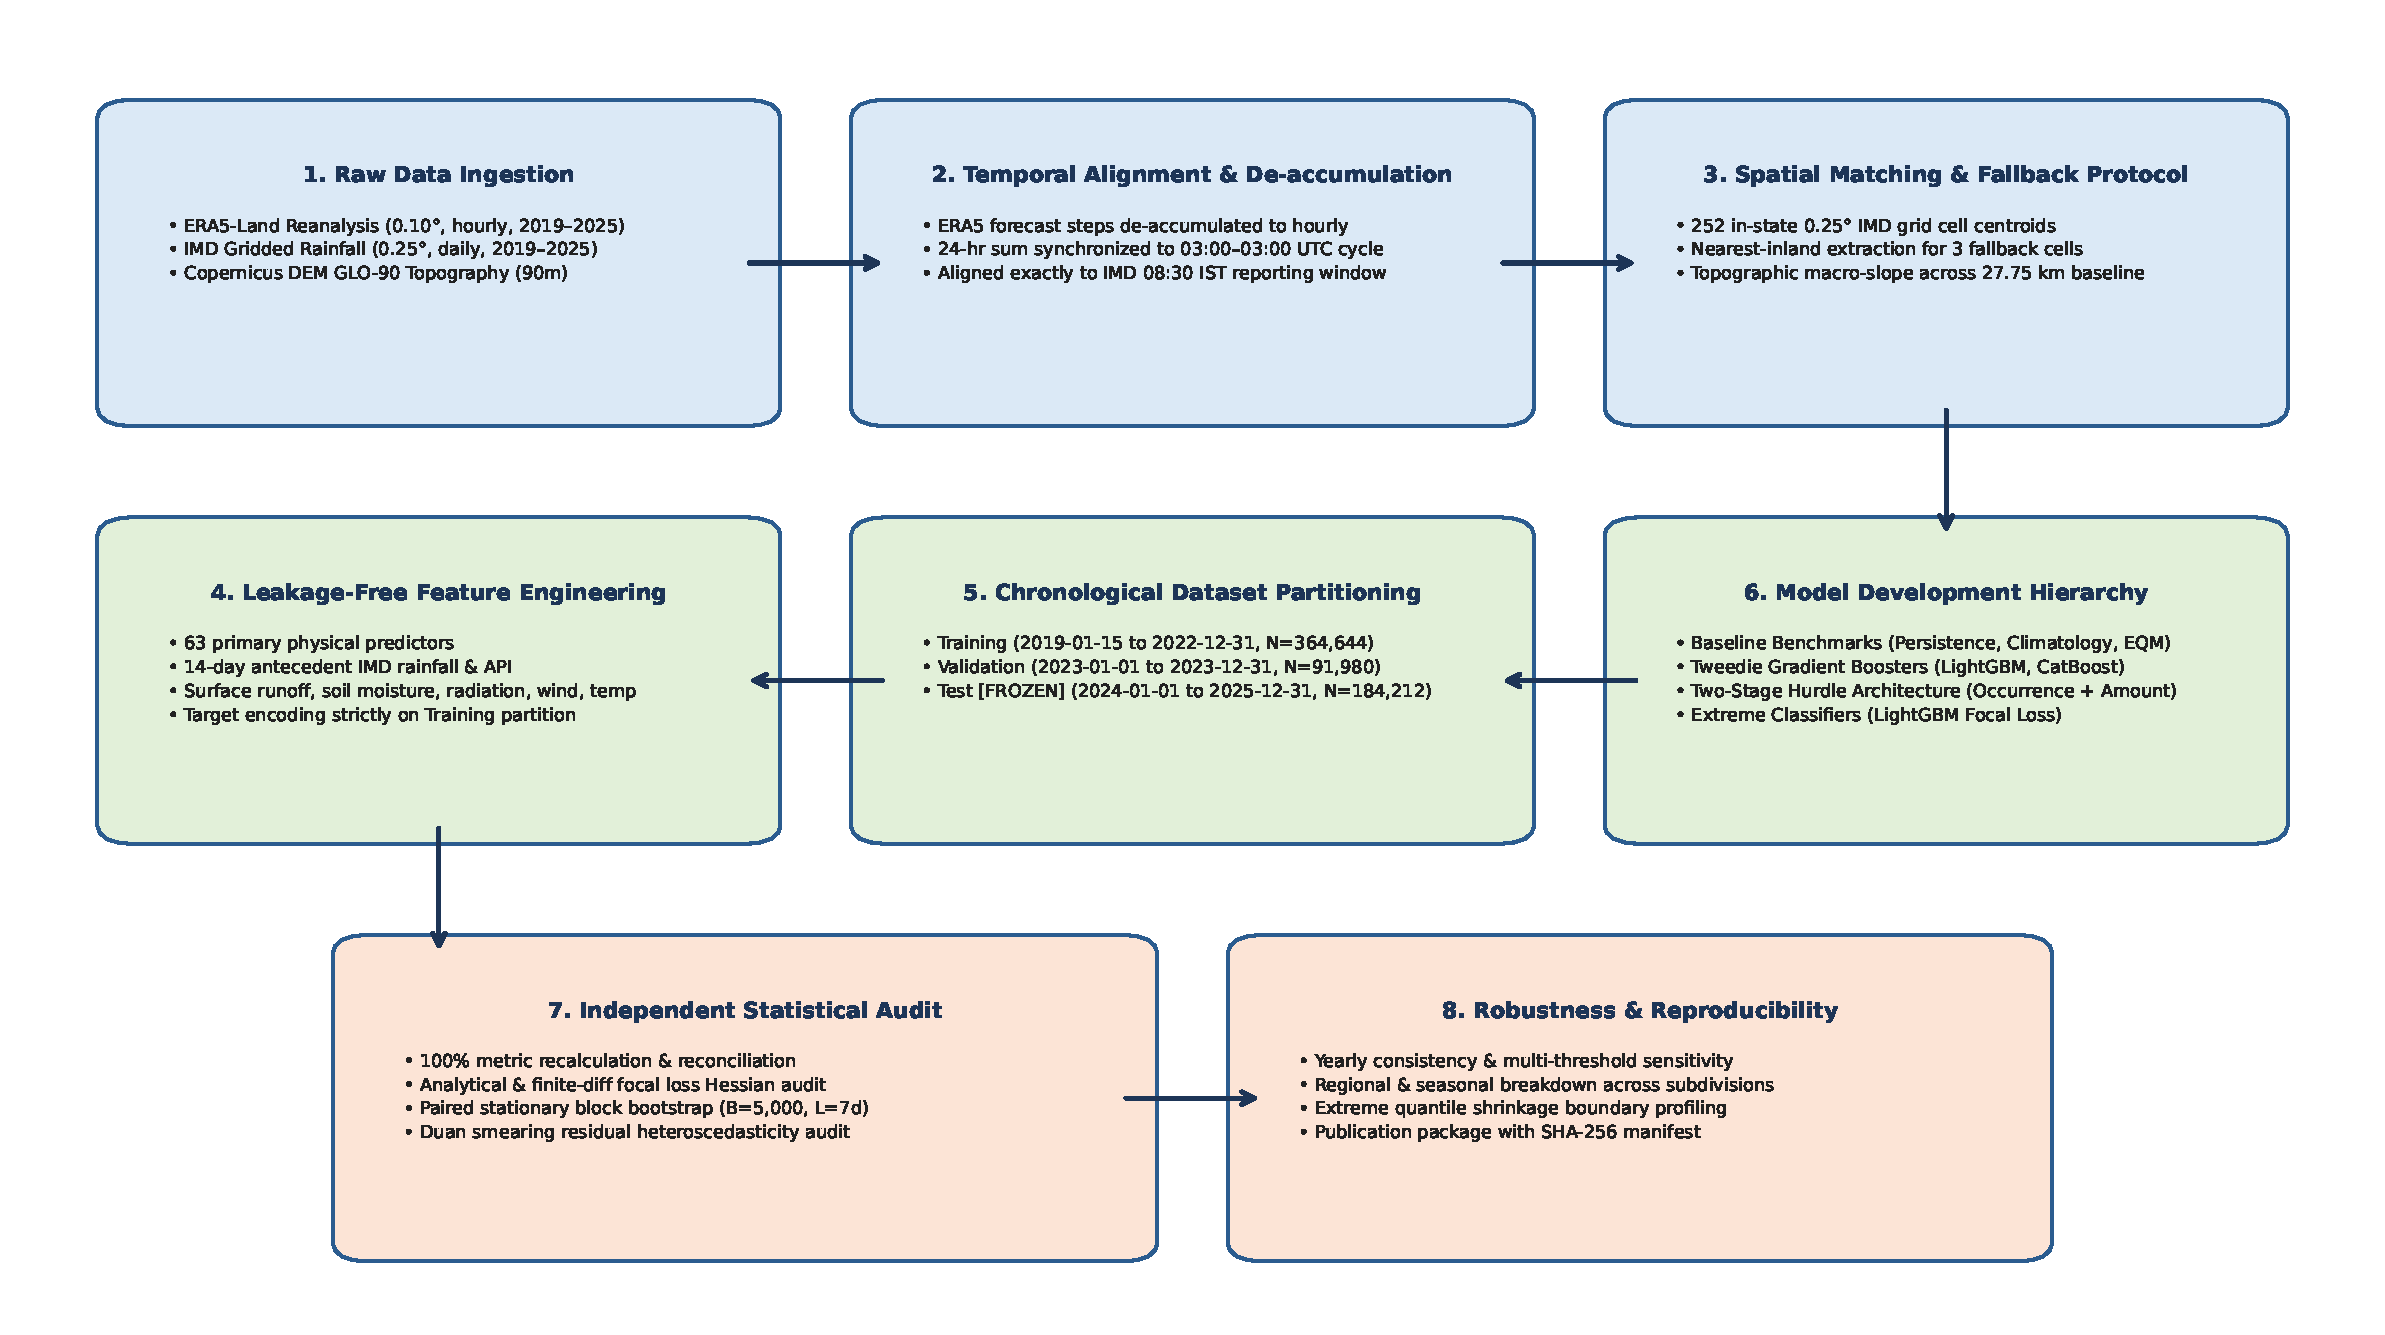
\includegraphics[width=0.88\textwidth]{figures/figure2_methodology}
\caption{End-to-end retrospective machine learning architecture depicting ERA5-Land flux de-accumulation, IMD gauge preparation, 24-h causal lag alignment, 63 primary feature engineering, temporal partitioning, model training, and multi-criteria evaluation.}
\label{fig:methodology}
\end{figure}

\subsection{Feature Matrix Architecture}
The final dataset schema comprises 78 columns: 4 ground-truth target labels, 4 geographic/administrative identifiers, 2 protocol metadata strings, 4 excluded atmospheric pressure proxies and seasonal strings, 1 auxiliary quality flag (\texttt{is\_coastal\_fallback}), and exactly \textbf{63 primary predictors} ($X$) respecting the 24-hour causal latency constraint ($T_{\text{issue}} = \text{03:00 UTC on day } t-1$).

In the training pipeline, the model input feature matrix $X$ is constructed by taking the 61 numeric primary features and transforming the 2 raw string categorical columns (\texttt{subdivision} and \texttt{zone\_id}) via target mean encoding fitted strictly on the 2019--2022 training partition (\texttt{subdiv\_map} and \texttt{zone\_map}). The resulting numerical features (\texttt{subdivision\_enc} and \texttt{zone\_id\_enc}) replace the raw string fields in the model matrix, yielding an exact 63-column numerical matrix ($X \in \mathbb{R}^{N \times 63}$) fed to the gradient-boosted decision trees and linear models without future target leakage.

As structured in Table~\ref{tab:features}, these 63 primary model predictors span seven physical and hydrometeorological domains:
\begin{enumerate}
    \item \textbf{Antecedent IMD Rainfall Memory (13 features):} Lagged local ground-truth rainfall ($y_{t-1}, y_{t-2}, y_{t-3}, y_{t-7}, y_{t-14}$), rolling window sums and means (3-day, 7-day, 14-day), 7-day rolling maximum, and the 14-day Antecedent Precipitation Index ($\text{API}_{14} = \sum_{k=1}^{14} 0.85^k y_{t-k}$), all shifted strictly by $\ge 1\text{ day}$.
    \item \textbf{ERA5-Land Precipitation \& Hydrological Balance (14 features):} Antecedent reanalysis total precipitation (\texttt{era5\_tp\_lag\_1d}, \texttt{\_lag\_2d}, \texttt{\_lag\_3d}, 3-day and 7-day rolling sums), land-surface runoff fluxes (\texttt{ro\_lag\_1d}, \texttt{sro\_lag\_1d}), canopy skin reservoir storage (\texttt{src\_lag\_1d}), evaporation components (\texttt{e\_lag\_1d}, \texttt{pev\_lag\_1d}, \texttt{evabs\_lag\_1d}, \texttt{evatc\_lag\_1d}, \texttt{evavt\_lag\_1d}), and surface albedo (\texttt{fal\_lag\_1d}).
    \item \textbf{Atmospheric Thermodynamic State \& Wind (12 features):} 2-meter air temperature dynamics (\texttt{t2m\_mean\_lag\_1d}, \texttt{t2m\_min\_lag\_1d}, \texttt{t2m\_max\_lag\_1d}, diurnal range \texttt{temp\_range\_lag\_1d}, 3-day and 7-day rolling means), moisture saturation diagnostics (\texttt{d2m\_mean\_lag\_1d}, dewpoint depression \texttt{dewpoint\_depression\_lag\_1d}), surface pressure (\texttt{sp\_lag\_1d}), and 10-meter wind speed dynamics (\texttt{wind\_speed\_lag\_1d}, 3-day and 7-day rolling means).
    \item \textbf{Soil Moisture Profiles \& Radiative/Turbulent Energy Fluxes (9 features):} Multi-layer volumetric soil water content (\texttt{swvl1\_lag\_1d} for 0--7~cm depth, \texttt{swvl1\_lag\_3d}, \texttt{swvl1\_lag\_7d}, \texttt{swvl2\_lag\_1d} for 7--28~cm, \texttt{swvl3\_lag\_1d} for 28--100~cm), surface solar radiation downwards (\texttt{ssrd\_lag\_1d}), surface thermal radiation downwards (\texttt{strd\_lag\_1d}), surface latent heat flux (\texttt{slhf\_lag\_1d}), and surface sensible heat flux (\texttt{sshf\_lag\_1d}).
    \item \textbf{Static Topography, Elevation \& Spatial Proximity (6 features):} Terrain elevation from Copernicus GLO-90 DEM (\texttt{elevation\_dem\_m}), local terrain slope (\texttt{slope\_dem\_deg}), shortest Euclidean distance to the Arabian Sea coastline (\texttt{dist\_to\_coast\_km}), orthogonal distance to the Western Ghats mountain crest line (\texttt{dist\_to\_ghats\_crest\_km}), and IMD 0.25$^\circ$ grid-cell centroid geographic coordinates (\texttt{latitude}, \texttt{longitude}).
    \item \textbf{Cyclic Temporal Ephemeris \& Astronomical Cycles (7 features):} Calendar month, Julian day of year, harmonic cyclical expansions ($\sin(2\pi \cdot \text{DOY}/366)$, $\cos(2\pi \cdot \text{DOY}/366)$, $\sin(2\pi \cdot \text{Month}/12)$, $\cos(2\pi \cdot \text{Month}/12)$), and Southwest monsoon seasonal indicator (\texttt{is\_monsoon}).
    \item \textbf{Primary Regional Categorical Encodings (2 features):} Out-of-sample target-encoded regional indicators (\texttt{subdivision\_enc} for the 4 meteorological subdivisions and \texttt{zone\_id\_enc} for the 10 agroclimatic zones), which replace the raw categorical string columns in the model feature matrix.
\end{enumerate}

\begin{table*}[htbp]
\centering
\caption{Input Feature Groups, Predictor Schema, and Pipeline Causal Gating (63 Primary Features)}
\label{tab:features}
\resizebox{\textwidth}{!}{
\begin{tabular}{p{3.5cm}cp{5.5cm}p{4cm}p{5.5cm}}
\toprule
\textbf{Feature Group} & \textbf{Predictor Count} & \textbf{Representative Variables} & \textbf{Temporal Alignment} & \textbf{Scientific Relevance} \\
\midrule
1. Antecedent IMD Rainfall Memory & 13 & target\_rain\_lag\_1d, lag\_2d, lag\_3d, lag\_7d, lag\_14d, roll\_3d\_sum, roll\_7d\_sum, roll\_14d\_sum, roll\_3d\_mean, roll\_7d\_mean, roll\_14d\_mean, roll\_7d\_max, api\_14d & 03:00 UTC Day d-1 (Lag 1) to Day d-14 (all shifted strictly by $\ge$1 day) & Ground-truth antecedent precipitation persistence, catchment moisture memory, and 14-day antecedent precipitation index (decay k=0.85). \\
2. ERA5-Land Precipitation \& Hydrological Balance & 14 & era5\_tp\_lag\_1d, lag\_2d, lag\_3d, roll\_3d\_sum, roll\_7d\_sum, ro\_lag\_1d (total runoff), sro\_lag\_1d (surface runoff), src\_lag\_1d (skin reservoir), e\_lag\_1d, pev\_lag\_1d, evabs\_lag\_1d, evatc\_lag\_1d, evavt\_lag\_1d, fal\_lag\_1d & De-accumulated daily sum 04:00 UTC Day d-2 to 03:00 UTC Day d-1 (Lag 1) & Antecedent reanalysis-derived precipitation and land-surface flux memory, model-derived runoff proxies of soil saturation, canopy interception storage, and evapotranspiration demand. \\
3. Atmospheric Thermodynamic State \& Wind & 12 & t2m\_mean\_lag\_1d, t2m\_min\_lag\_1d, t2m\_max\_lag\_1d, temp\_range\_lag\_1d, d2m\_mean\_lag\_1d, dewpoint\_depression\_lag\_1d, t2m\_roll\_3d\_mean, t2m\_roll\_7d\_mean, sp\_lag\_1d, wind\_speed\_lag\_1d, wind\_roll\_3d\_mean, wind\_roll\_7d\_mean & Daily mean, min, max over 24-hr cycle ending 03:00 UTC Day d-1 & Boundary-layer thermal structure, moisture saturation deficit (sub-cloud relative humidity proxy), synoptic surface pressure, and near-surface 10-meter wind speed circulation conditions. \\
4. Soil Moisture Profiles \& Radiative/Turbulent Fluxes & 9 & swvl1\_lag\_1d (0-7 cm), swvl1\_lag\_3d, swvl1\_lag\_7d, swvl2\_lag\_1d (7-28 cm), swvl3\_lag\_1d (28-100 cm), ssrd\_lag\_1d (solar), strd\_lag\_1d (thermal), slhf\_lag\_1d (latent), sshf\_lag\_1d (sensible) & Layer volumetric water content and daily accumulated radiative/turbulent energy fluxes ending 03:00 UTC Day d-1 & Root-zone soil water storage, cloud-cover radiative trapping (downward longwave), clear-sky solar insolation, and surface sensible/latent heat partitioning. \\
5. Topography, Elevation \& Spatial Proximity & 6 & elevation\_dem\_m, slope\_dem\_deg, latitude, longitude, dist\_to\_coast\_km, dist\_to\_ghats\_crest\_km & Static spatial coordinates and Copernicus DEM GLO-90 terrain metrics & Orographic uplift forcing along the Western Ghats barrier, maritime-continental continentality gradient, and regional terrain slope gradient. \\
6. Temporal Ephemeris \& Astronomical Cycles & 7 & month, day\_of\_year, sin\_day\_of\_year, cos\_day\_of\_year, sin\_month, cos\_month, is\_monsoon & Harmonic cyclical transformation of Julian date and calendar indicators known at issue time & Synoptic seasonal climatology, solar declination angle, and Southwest Monsoon boundary definition. \\
7. Primary Categorical Regional Predictors & 2 & subdivision (Coastal Karnataka, Malnad, North Interior, South Interior), zone\_id (10 agroclimatic zones) [target-encoded into subdivision\_enc, zone\_id\_enc] & Static administrative / agroclimatic classification (target encoding fitted strictly on Training partition) & Regional agroclimatic baselines and spatial climatological stratification. \\
Auxiliary Quality Flag (Separate from Primary Predictors) & 1 & is\_coastal\_fallback (binary 0/1 indicator for Grid-Cell IDs 52, 68, 125) & Static data-quality indicator & Flags coastal cells touching ocean boundaries requiring nearest-land neighbor fallback extraction. \\
\bottomrule
\end{tabular}
}
\end{table*}

\subsection{Model Formulations Across Tiers}
We implement a hierarchical modeling framework across five structural tiers:
\begin{itemize}
    \item \textbf{Tier 0 (Naive Baselines):} Persistence ($y_t = y_{t-1}$) and Grid-Cell DOY Climatology (historical day-of-year mean per grid cell).
    \item \textbf{Tier 1 (Raw Reanalysis Benchmark):} Uncalibrated antecedent ERA5-Land precipitation.
    \item \textbf{Tier 2 (Statistical Downscaling):} Empirical Quantile Mapping (EQM) \cite{piani2011} using 100 empirical quantile knots fitted per IMD grid cell on 2019--2022.
    \item \textbf{Tier 3 (Regularized Linear Baselines):} Ridge Regression (L2 regularization, $\alpha = 100.0$) and ElasticNet Regression ($\alpha = 0.1$, $\text{l1\_ratio} = 0.5$) fitted on standardized features.
    \item \textbf{Tier 4 (Machine Learning Architectures):} LightGBM Tweedie ($p=1.5$) \cite{ke2017, tweedie1984, dunn2005}, CatBoost Tweedie ($p=1.5$) \cite{prokhorenkova2018}, XGBoost Tweedie \cite{chen2016}, LightGBM Log-Ordinary with Duan Smearing \cite{duan1983}, and a Two-Stage Hurdle Model combining binary rain occurrence classification (LGBM logistic) with truncated regression (LGBM Gamma GLM) \cite{cragg1971}.
\end{itemize}

\subsection{Dedicated Heavy Rainfall Classification \& Custom Asymmetric Focal Loss}
Because extreme rainfall events ($\ge 64.5$\;mm/day) constitute only $0.6878\%$ of test records, standard binary cross-entropy produces prohibitive miss rates. We implement an experimental custom Lin et al. \cite{lin2017} Focal Loss objective in LightGBM with focusing parameter $\gamma = 2.0$ and $\alpha$-balancing = 0.75:
\begin{equation}
\text{FL}(p_t) = -\alpha_t (1 - p_t)^\gamma \log(p_t)
\end{equation}
The first- and second-order custom gradients were analytically derived. The validation-selected decision threshold $p^* = 0.53$ was chosen strictly on the 2023 validation partition to maximize the Critical Success Index (CSI). It represents an empirical decision boundary rather than a calibrated posterior probability.

\subsection{Evaluation Metrics \& Paired Stationary Block Bootstrapping}
Continuous performance is evaluated using RMSE, MAE, Mean Bias, Percentage Bias (PBias), Pearson correlation ($r$), Nash-Sutcliffe Efficiency (NSE) \cite{nash1970}, Classic KGE-2009 \cite{gupta2009}, and Modified KGE-2012 \cite{kling2012}. Categorical heavy rain alerting is evaluated via Hits ($H$), Misses ($M$), False Alarms ($F$), Correct Negatives ($C$), Probability of Detection (POD / Recall), False Alarm Ratio (FAR), Precision, Critical Success Index (CSI / Threat Score), Heidke Skill Score (HSS), and Equitable Threat Score (ETS).

To account for spatial cross-correlation across the 252 grid cells and temporal autocorrelation across consecutive days, we implement a stationary paired block bootstrap protocol \cite{kunsch1989, politis1994} with $B = 2,000$ resamples under block lengths $L = 7\text{ days}$ (synoptic weather cycle) and $L = 14\text{ days}$ (intraseasonal scale). The paired stationary block-bootstrap analysis provides strong statistical evidence of lower RMSE under the evaluated resampling assumptions (empirical resolution $p < 0.0005$).

\section{Results}\label{sec4}

\subsection{Continuous Rainfall Estimation \& Multi-Criteria Benchmarking}
Table~\ref{tab:benchmarking} presents out-of-sample forward evaluation on the frozen 2024--2025 test partition ($N = 184,212$ instances). Rather than demonstrating a single universally dominant architecture, the three gradient-boosted models exhibit competitive performance characterized by distinct multi-criteria trade-offs:
\begin{itemize}
    \item \textbf{Hurdle Expected Value} achieves the lowest overall RMSE ($7.4241$\;mm), highest Pearson correlation ($r = 0.7380$), and highest Nash-Sutcliffe Efficiency ($\text{NSE} = 0.5443$).
    \item \textbf{CatBoost Tweedie} attains the highest Modified Kling-Gupta Efficiency ($\text{KGE-2012} = 0.6261$) with $\text{RMSE} = 7.4335$\;mm and $\text{MAE} = 2.9186$\;mm.
    \item \textbf{LightGBM Tweedie} achieves the lowest Mean Absolute Error ($\text{MAE} = 2.8993$\;mm) and lowest mean bias ($-0.0179$\;mm, or $-0.51\%$ relative bias).
\end{itemize}

All three gradient-boosted architectures substantially outperform naive Persistence ($\text{RMSE} = 10.3582$\;mm; $-2.93$\;mm reduction), raw uncalibrated ERA5-Land ($\text{RMSE} = 10.4550$\;mm; $-3.03$\;mm reduction), and grid-cell-wise Empirical Quantile Mapping (EQM, $\text{RMSE} = 11.1970$\;mm, $\text{NSE} = -0.0366$) (Fig.~\ref{fig:hexbin} and Fig.~\ref{fig:benchmarking}).

\begin{table*}[htbp]
\centering
\caption{Comprehensive Out-of-Sample Model Benchmarking Portfolio (Test Partition 2024--2025; $N = 184,212$)}
\label{tab:benchmarking}
\resizebox{\textwidth}{!}{
\begin{tabular}{lllr r r r r r r r r}
\toprule
\textbf{Model Hierarchy Tier} & \textbf{Model Name} & \textbf{Loss Objective} & \textbf{RMSE mm} & \textbf{MAE mm} & \textbf{Mean Bias mm} & \textbf{PBias pct} & \textbf{Pearson r} & \textbf{NSE} & \textbf{Classic KGE 2009} & \textbf{Modified KGE 2012} & \textbf{Heavy CSI 64.5mm} \\
\midrule
Tier 0 (Naive Baselines) & Rainfall Persistence & Zero Learning & 10.3582 & 3.7508 & 0.0 & 0.0 & 0.5565 & 0.1129 & 0.5565 & 0.5565 & 0.2361 \\
Tier 0 (Naive Baselines) & Grid-cell DOY Climatology & Zero Learning & 10.1155 & 4.3078 & 0.2296 & 6.54 & 0.4313 & 0.154 & 0.3068 & 0.2851 & 0.0144 \\
Tier 1 (Raw Reanalysis) & Antecedent ERA5-Land Total Precip & Zero Learning & 10.455 & 4.1416 & 0.556 & 15.85 & 0.4911 & 0.0963 & 0.451 & 0.4111 & 0.1233 \\
Tier 2 (Statistical Downscaling) & Empirical Quantile Mapping (EQM) & Non-Parametric Knots & 11.197 & 4.2117 & 0.3867 & 11.02 & 0.4941 & -0.0366 & 0.4818 & 0.4763 & 0.1969 \\
Tier 3 (Linear Baselines) & Ridge Regression & L2 Regularized Linear & 7.975 & 3.3905 & 0.3308 & 9.43 & 0.6894 & 0.4742 & 0.5613 & 0.5184 & 0.2299 \\
Tier 3 (Linear Baselines) & ElasticNet Regression & L1/L2 Regularized Linear & 8.0156 & 3.3999 & 0.3034 & 8.65 & 0.6853 & 0.4688 & 0.5496 & 0.5101 & 0.2211 \\
Tier 4 (Machine Learning) & LightGBM RMSE & RMSE (L2) & 7.4982 & 3.0806 & 0.2698 & 7.69 & 0.732 & 0.5352 & 0.619 & 0.5812 & 0.3016 \\
Tier 4 (Machine Learning) & LightGBM Log OrdinaryInverse & Log MSE & 7.8497 & 2.615 & -1.3274 & -37.83 & 0.726 & 0.4906 & 0.3703 & 0.5276 & 0.2271 \\
Tier 4 (Machine Learning) & LightGBM Log DuanSmearing & Log MSE & 7.5893 & 2.9488 & -0.2105 & -6.0 & 0.726 & 0.5238 & 0.6439 & 0.6722 & 0.3509 \\
Tier 4 (Machine Learning) & LightGBM Tweedie p1.5 & Compound Poisson-Gamma (p=1.5) & 7.4427 & 2.8993 & -0.0179 & -0.51 & 0.7363 & 0.542 & 0.6218 & 0.6245 & 0.2868 \\
Tier 4 (Machine Learning) & CatBoost Tweedie p1.5 & Compound Poisson-Gamma (p=1.5) & 7.4335 & 2.9186 & 0.0388 & 1.11 & 0.737 & 0.5431 & 0.6318 & 0.6261 & 0.3033 \\
Tier 4 (Machine Learning) & Hurdle ExpectedValue & Two-Stage Hurdle Expected Value & 7.4241 & 2.93 & 0.0342 & 0.97 & 0.738 & 0.5443 & 0.6165 & 0.6114 & 0.3072 \\
\bottomrule
\end{tabular}
}
\end{table*}

\begin{figure}[htbp]
\centering
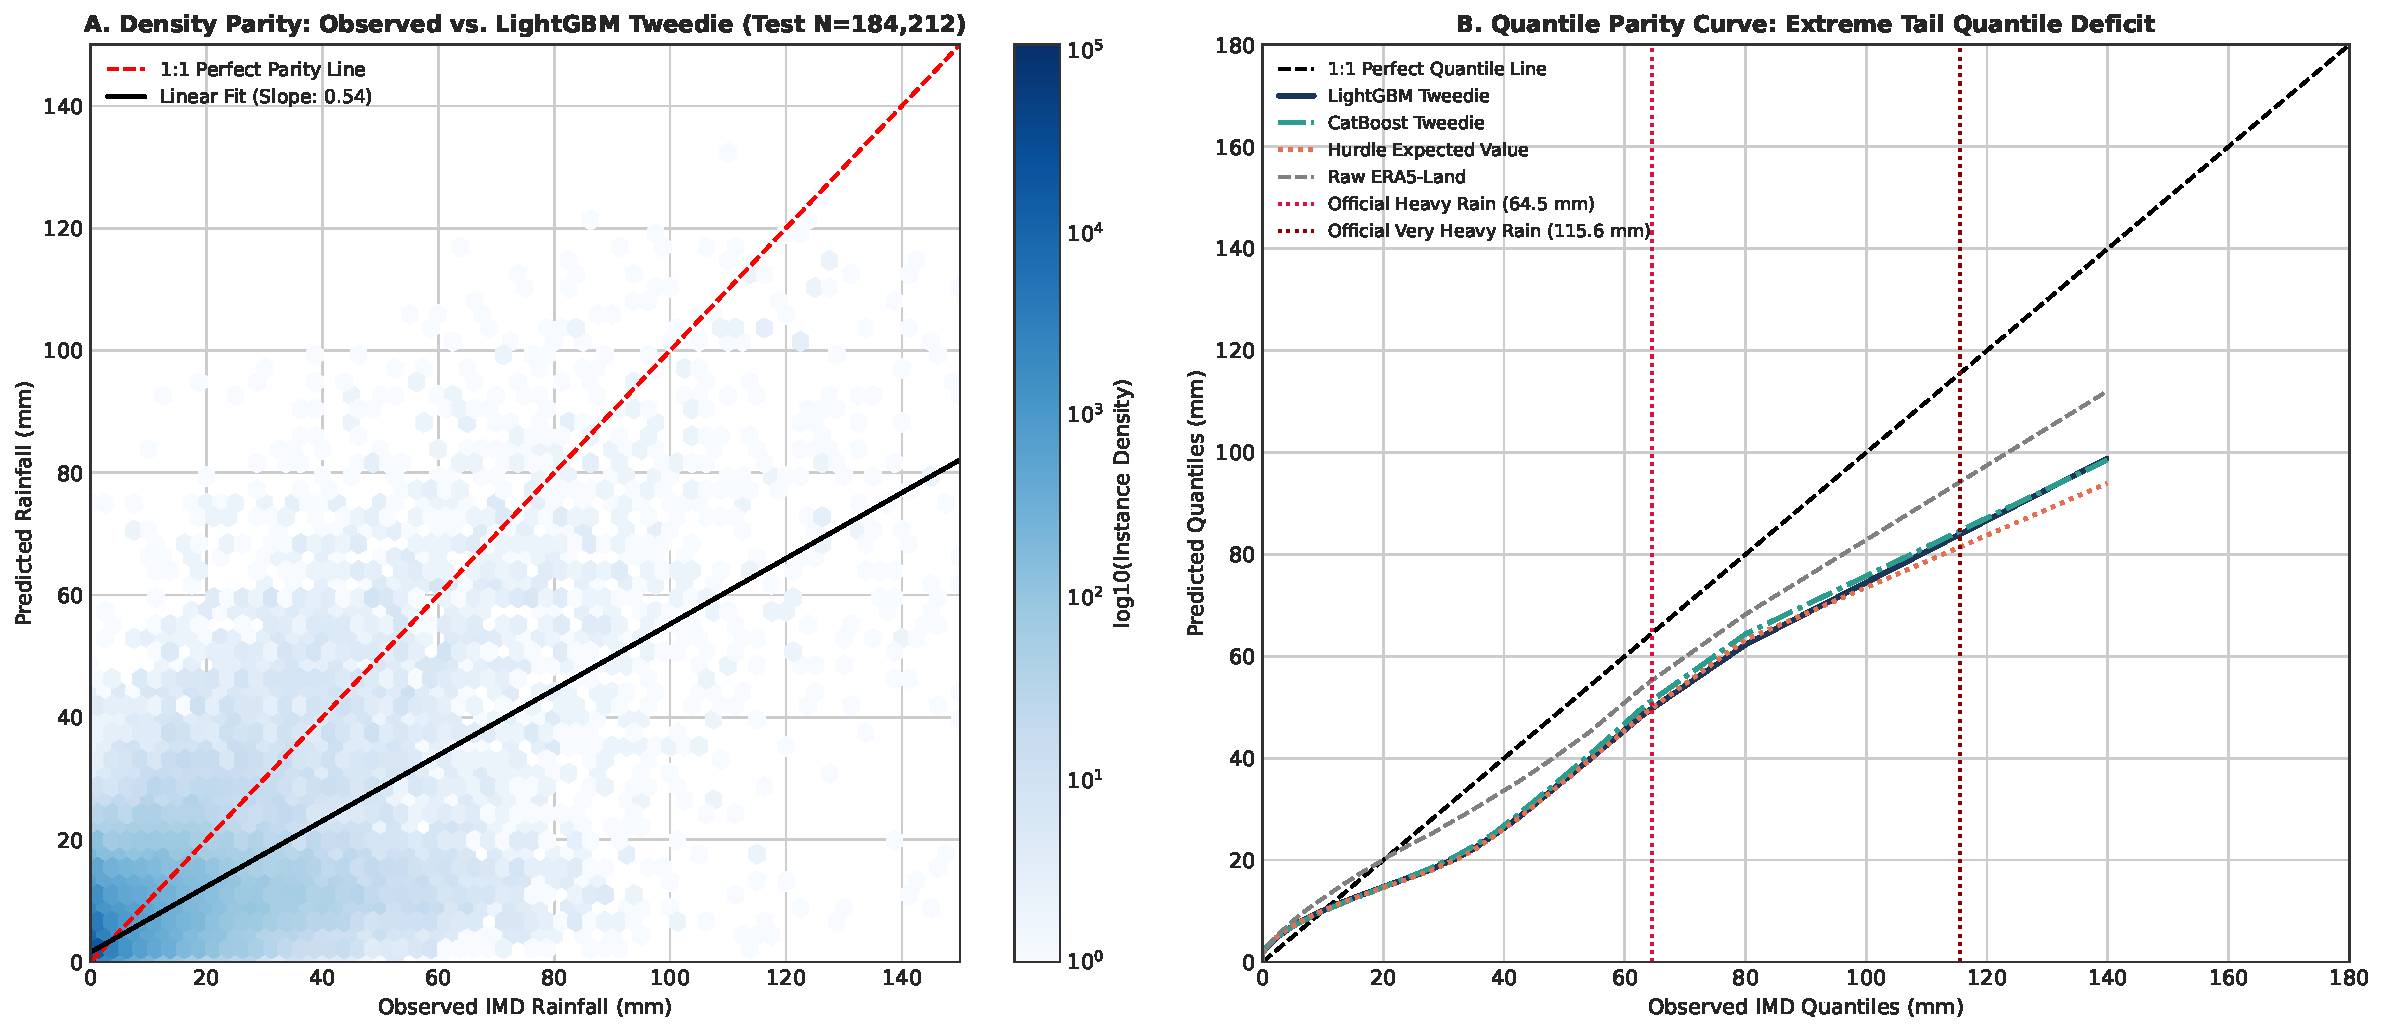
\includegraphics[width=0.72\textwidth]{figures/figure3_observed_predicted}
\caption{Density parity hexbin between observed and predicted daily rainfall on the 2024--2025 test partition. Color bar represents log-scaled instance density.}
\label{fig:hexbin}
\end{figure}

\begin{figure}[htbp]
\centering
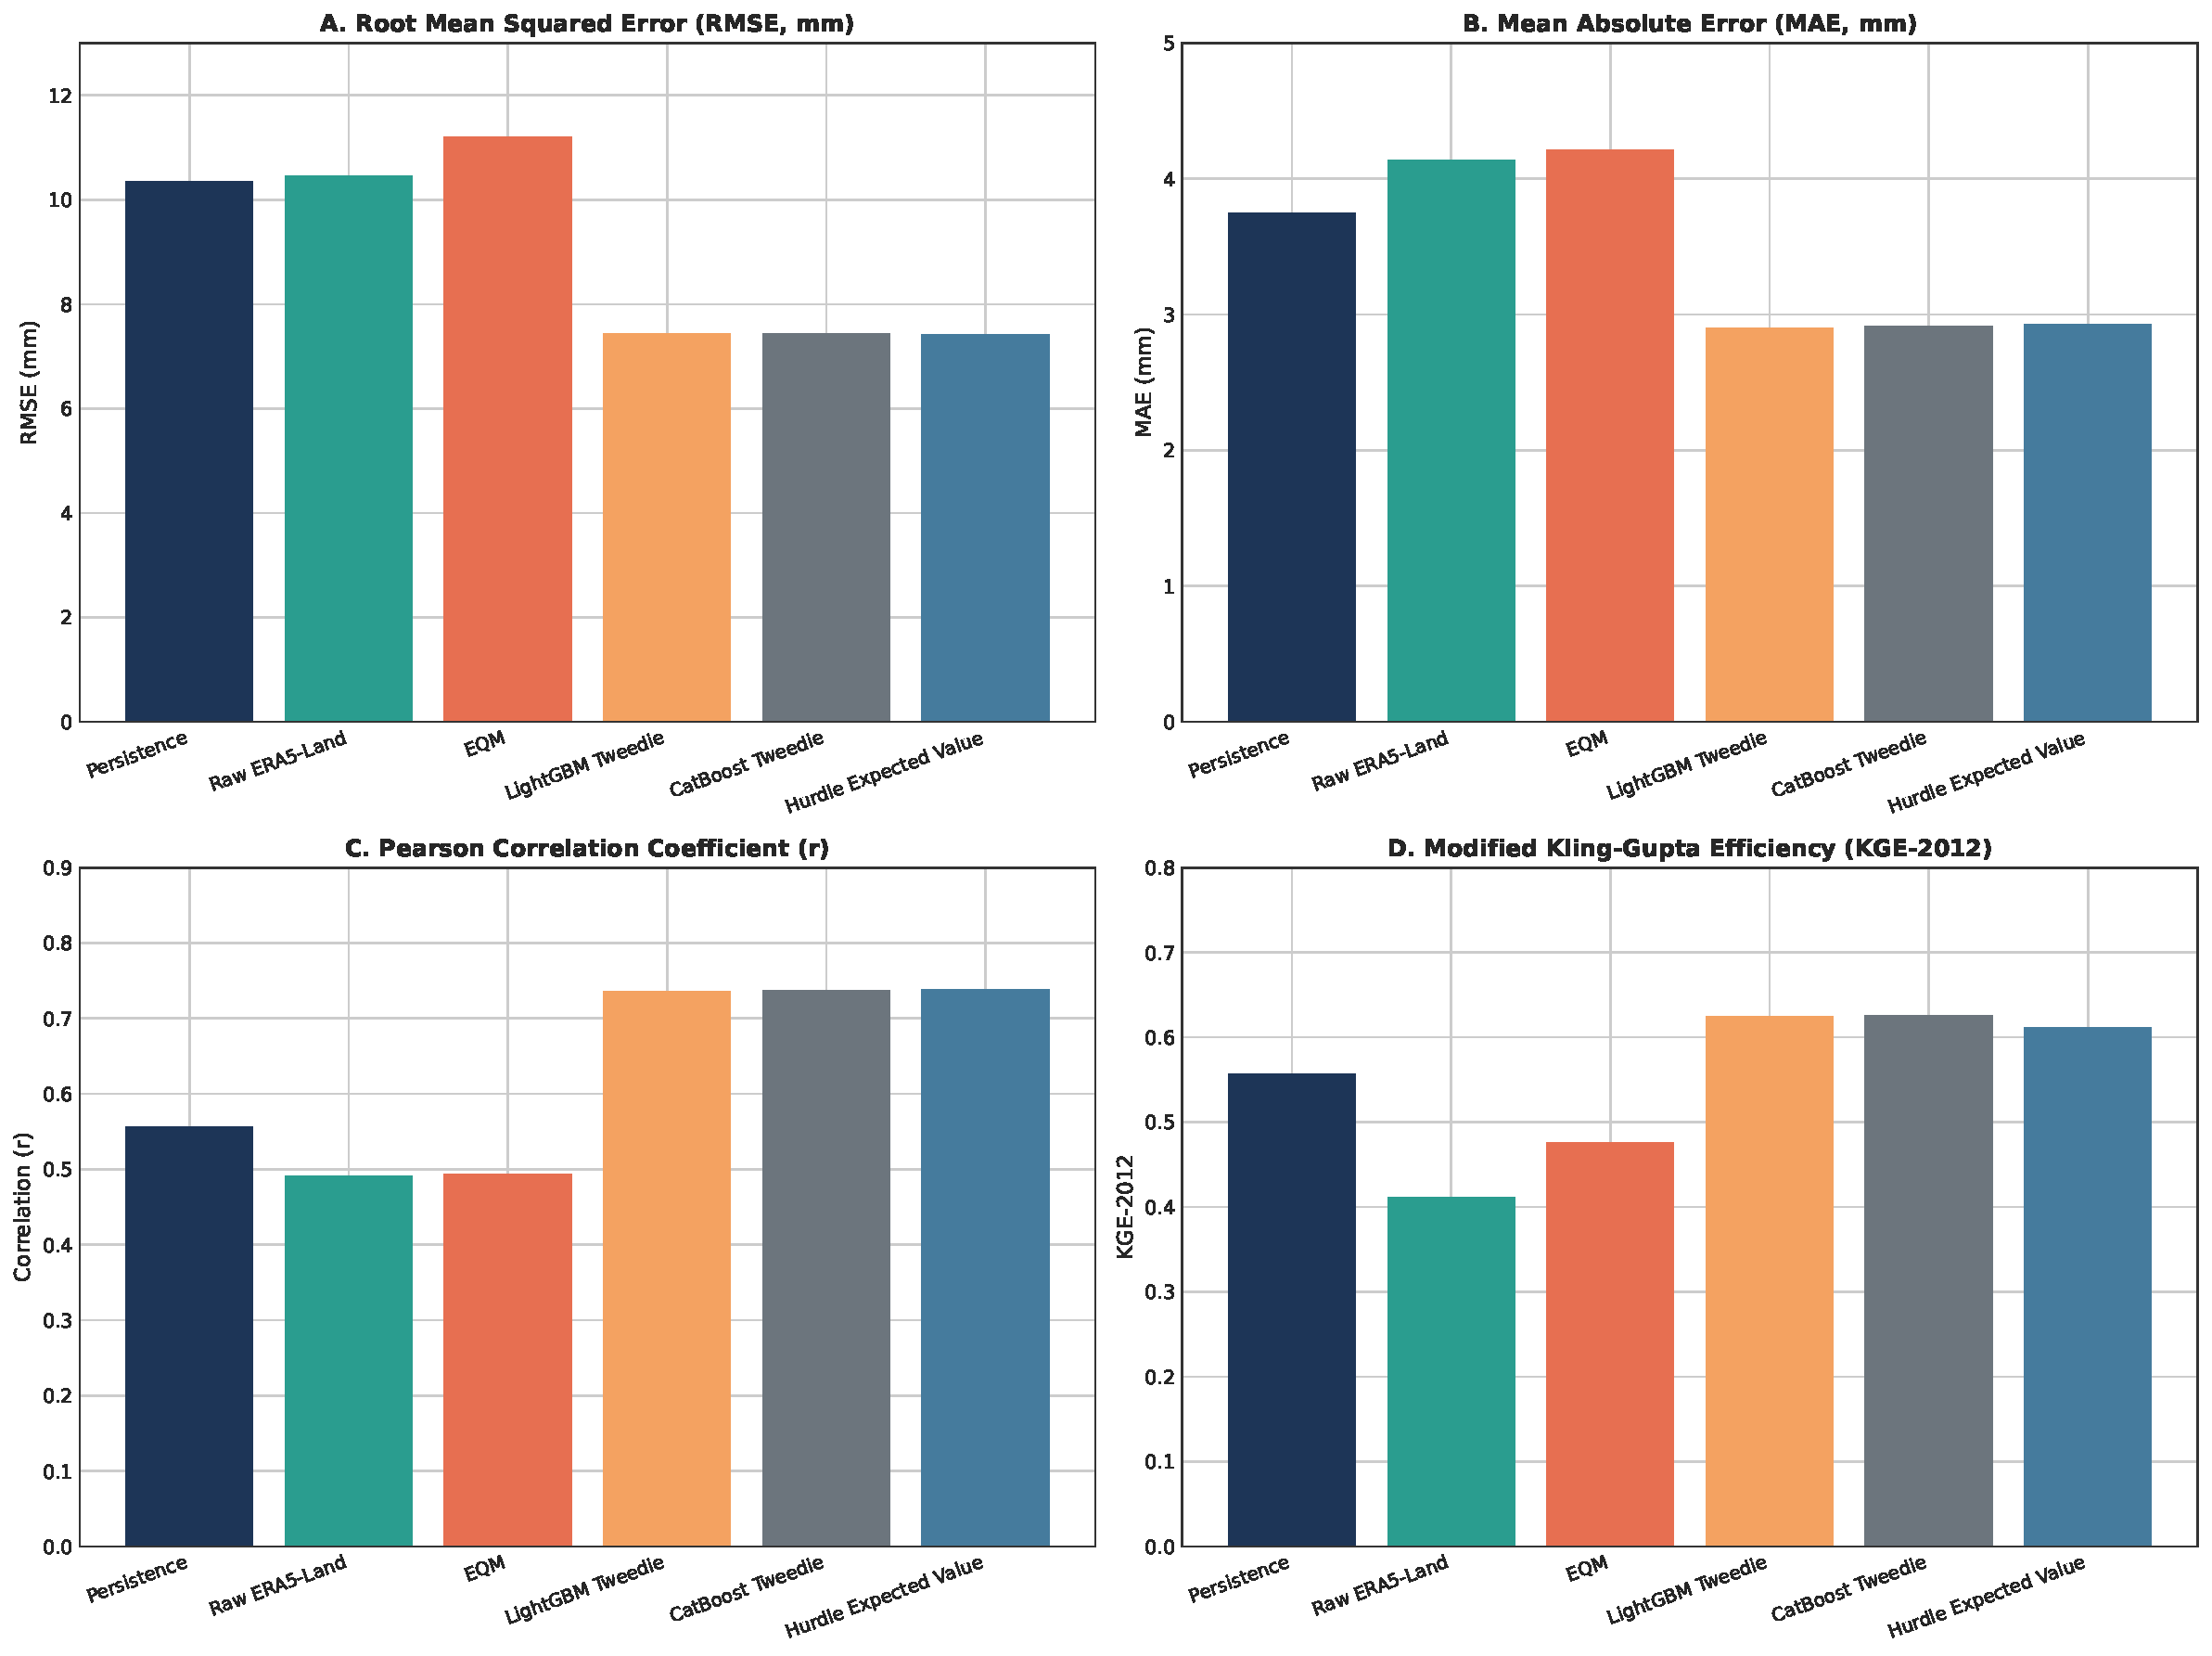
\includegraphics[width=0.88\textwidth]{figures/figure4_model_benchmarking}
\caption{Comparative bar panels showing RMSE, MAE, Pearson correlation, and KGE-2012 across all 11 evaluated models on the frozen test partition.}
\label{fig:benchmarking}
\end{figure}

\subsection{Heavy Rainfall Detection and Retrospective Classifier Evaluation}
Table~\ref{tab:heavy_rain} summarizes the performance of the dedicated heavy rainfall classification models for events $\ge 64.5$\;mm/day (1,267 true events out of 184,212 test records, prevalence = $0.6878\%$).

\begin{table*}[htbp]
\centering
\caption{Dedicated Heavy Rainfall ($\ge 64.5$\;mm) Contingency and Skill Score Evaluation (Test 2024--2025)}
\label{tab:heavy_rain}
\resizebox{\textwidth}{!}{
\begin{tabular}{llp{4.5cm}r r r r r r r r r r r}
\toprule
\textbf{Model Name} & \textbf{Decision Threshold} & \textbf{Threshold Selection Basis} & \textbf{Hits} & \textbf{Misses} & \textbf{False Alarms} & \textbf{Correct Negatives} & \textbf{Precision} & \textbf{POD Recall} & \textbf{FAR} & \textbf{CSI} & \textbf{HSS} & \textbf{ETS} & \textbf{PR AUC} \\
\midrule
LightGBM\_Heavy\_FocalLoss & 0.53 & Validation-selected decision threshold p*=0.53 chosen on 2023 Validation to maximize CSI & 595 & 672 & 427 & 182518 & 0.5822 & 0.4696 & 0.4178 & 0.3512 & 0.5169 & 0.3485 & 0.5084 \\
LightGBM\_Heavy\_ClassWeighted & 0.96 & Validation-selected decision threshold p*=0.96 chosen on 2023 Validation to maximize CSI & 688 & 579 & 722 & 182223 & 0.4879 & 0.543 & 0.5121 & 0.3459 & 0.5105 & 0.3427 & 0.4853 \\
CatBoost\_Heavy\_ClassWeighted & 0.98 & Validation-selected decision threshold p*=0.98 chosen on 2023 Validation to maximize CSI & 608 & 659 & 515 & 182430 & 0.5414 & 0.4799 & 0.4586 & 0.3412 & 0.5056 & 0.3383 & 0.4739 \\
Rainfall\_Persistence & 64.5 mm (fixed physical) & Physical 64.5 mm threshold applied directly to y\_{t-1} observations & 484 & 783 & 783 & 182162 & 0.382 & 0.382 & 0.618 & 0.2361 & 0.3777 & 0.2328 & nan \\
Raw\_ERA5\_Land & 64.5 mm (fixed physical) & Physical 64.5 mm threshold applied directly to raw antecedent total precipitation & 231 & 1036 & 606 & 182339 & 0.276 & 0.1823 & 0.724 & 0.1233 & 0.2153 & 0.1206 & nan \\
Empirical\_Quantile\_Mapping\_EQM & 64.5 mm (fixed physical) & Physical 64.5 mm threshold applied to grid-cell-specific quantile-mapped rainfall & 372 & 895 & 622 & 182323 & 0.3742 & 0.2936 & 0.6258 & 0.1969 & 0.325 & 0.194 & nan \\
\bottomrule
\end{tabular}
}
\end{table*}

\begin{figure}[htbp]
\centering
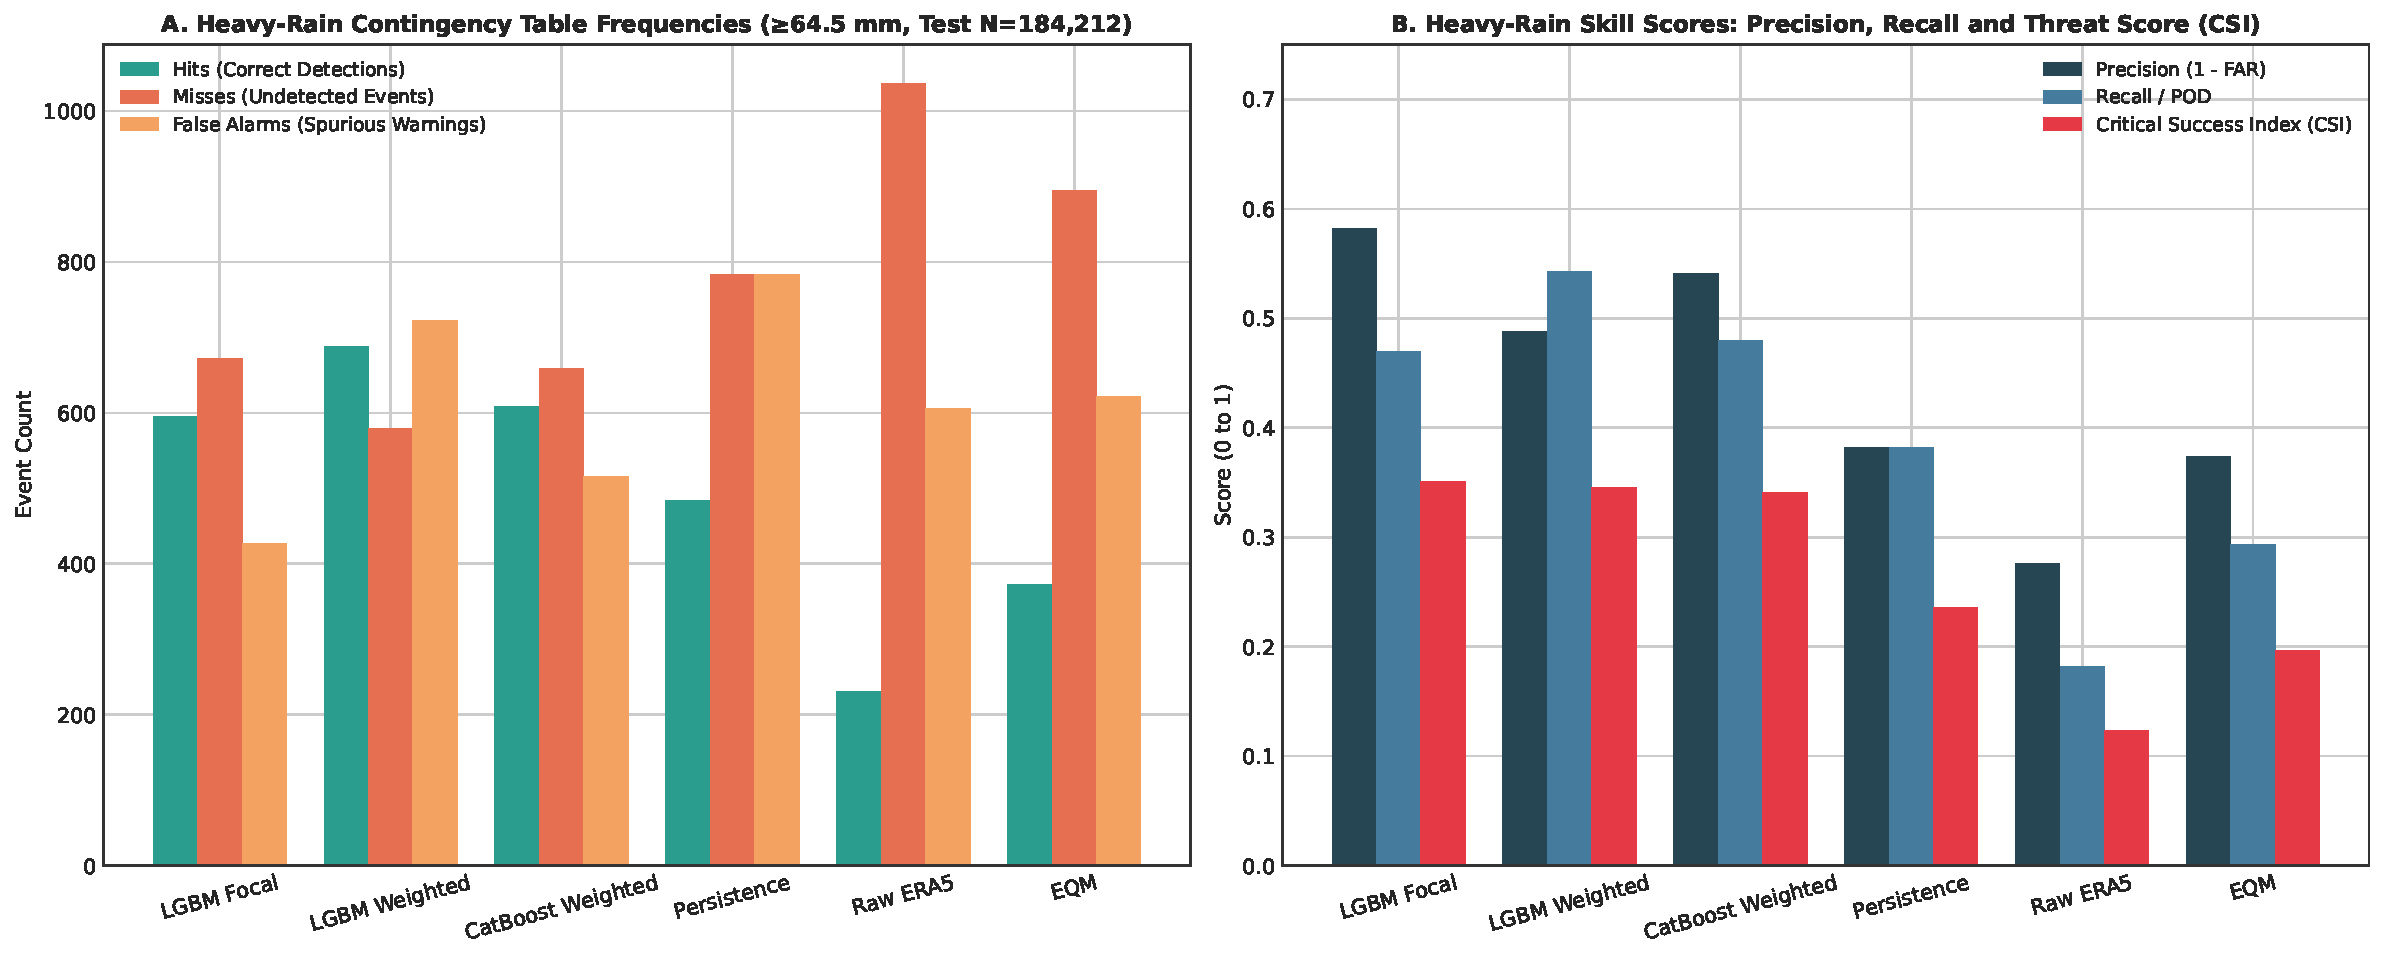
\includegraphics[width=0.85\textwidth]{figures/figure5_heavy_rain_detection}
\caption{Synoptic heavy-rain detection performance. Panel A shows contingency breakdown (Hits, Misses, False Alarms); Panel B shows Precision-Recall curves across classification architectures.}
\label{fig:heavy_rain}
\end{figure}

At the validation-selected decision threshold $p^* = 0.53$, the LightGBM Focal Loss classifier achieves a test POD of $46.96\%$ ($595$ hits), Precision of $58.22\%$, CSI of $0.3512$, and FAR of $41.78\%$ ($427$ false alarms), missing $53.04\%$ of observed heavy events ($672$ misses out of $1,267$) (Fig.~\ref{fig:heavy_rain}). Relative to standard class weighting, Focal Loss suppresses false alarms by $40.86\%$ ($427$ vs. $722$). However, because the model misses more than half of observed heavy events, it represents an experimental retrospective classification component rather than an operational flood warning system. Furthermore, this study does not establish reliable detection of very-heavy ($\ge 115.6$\;mm) or extremely-heavy ($\ge 204.5$\;mm) precipitation.

\subsection{Feature Attribution: Gain, Permutation, and Ablation Dynamics}
Figure~\ref{fig:attribution} and Table~\ref{tab:ablation} examine physical feature attribution and ablation dynamics across the 63 primary predictors. To avoid overconfident interpretation, we emphasize that tree split gain and permutation importance quantify empirical predictive sensitivity and variance reduction within the learned decision-tree ensemble \cite{breiman2001, fisher2019, lundberg2017}, rather than deterministic physical causality. Furthermore, the ablation scenarios reported on the 2024--2025 test partition are descriptive comparisons on the frozen test set without additional hypothesis testing.

\begin{figure}[htbp]
\centering
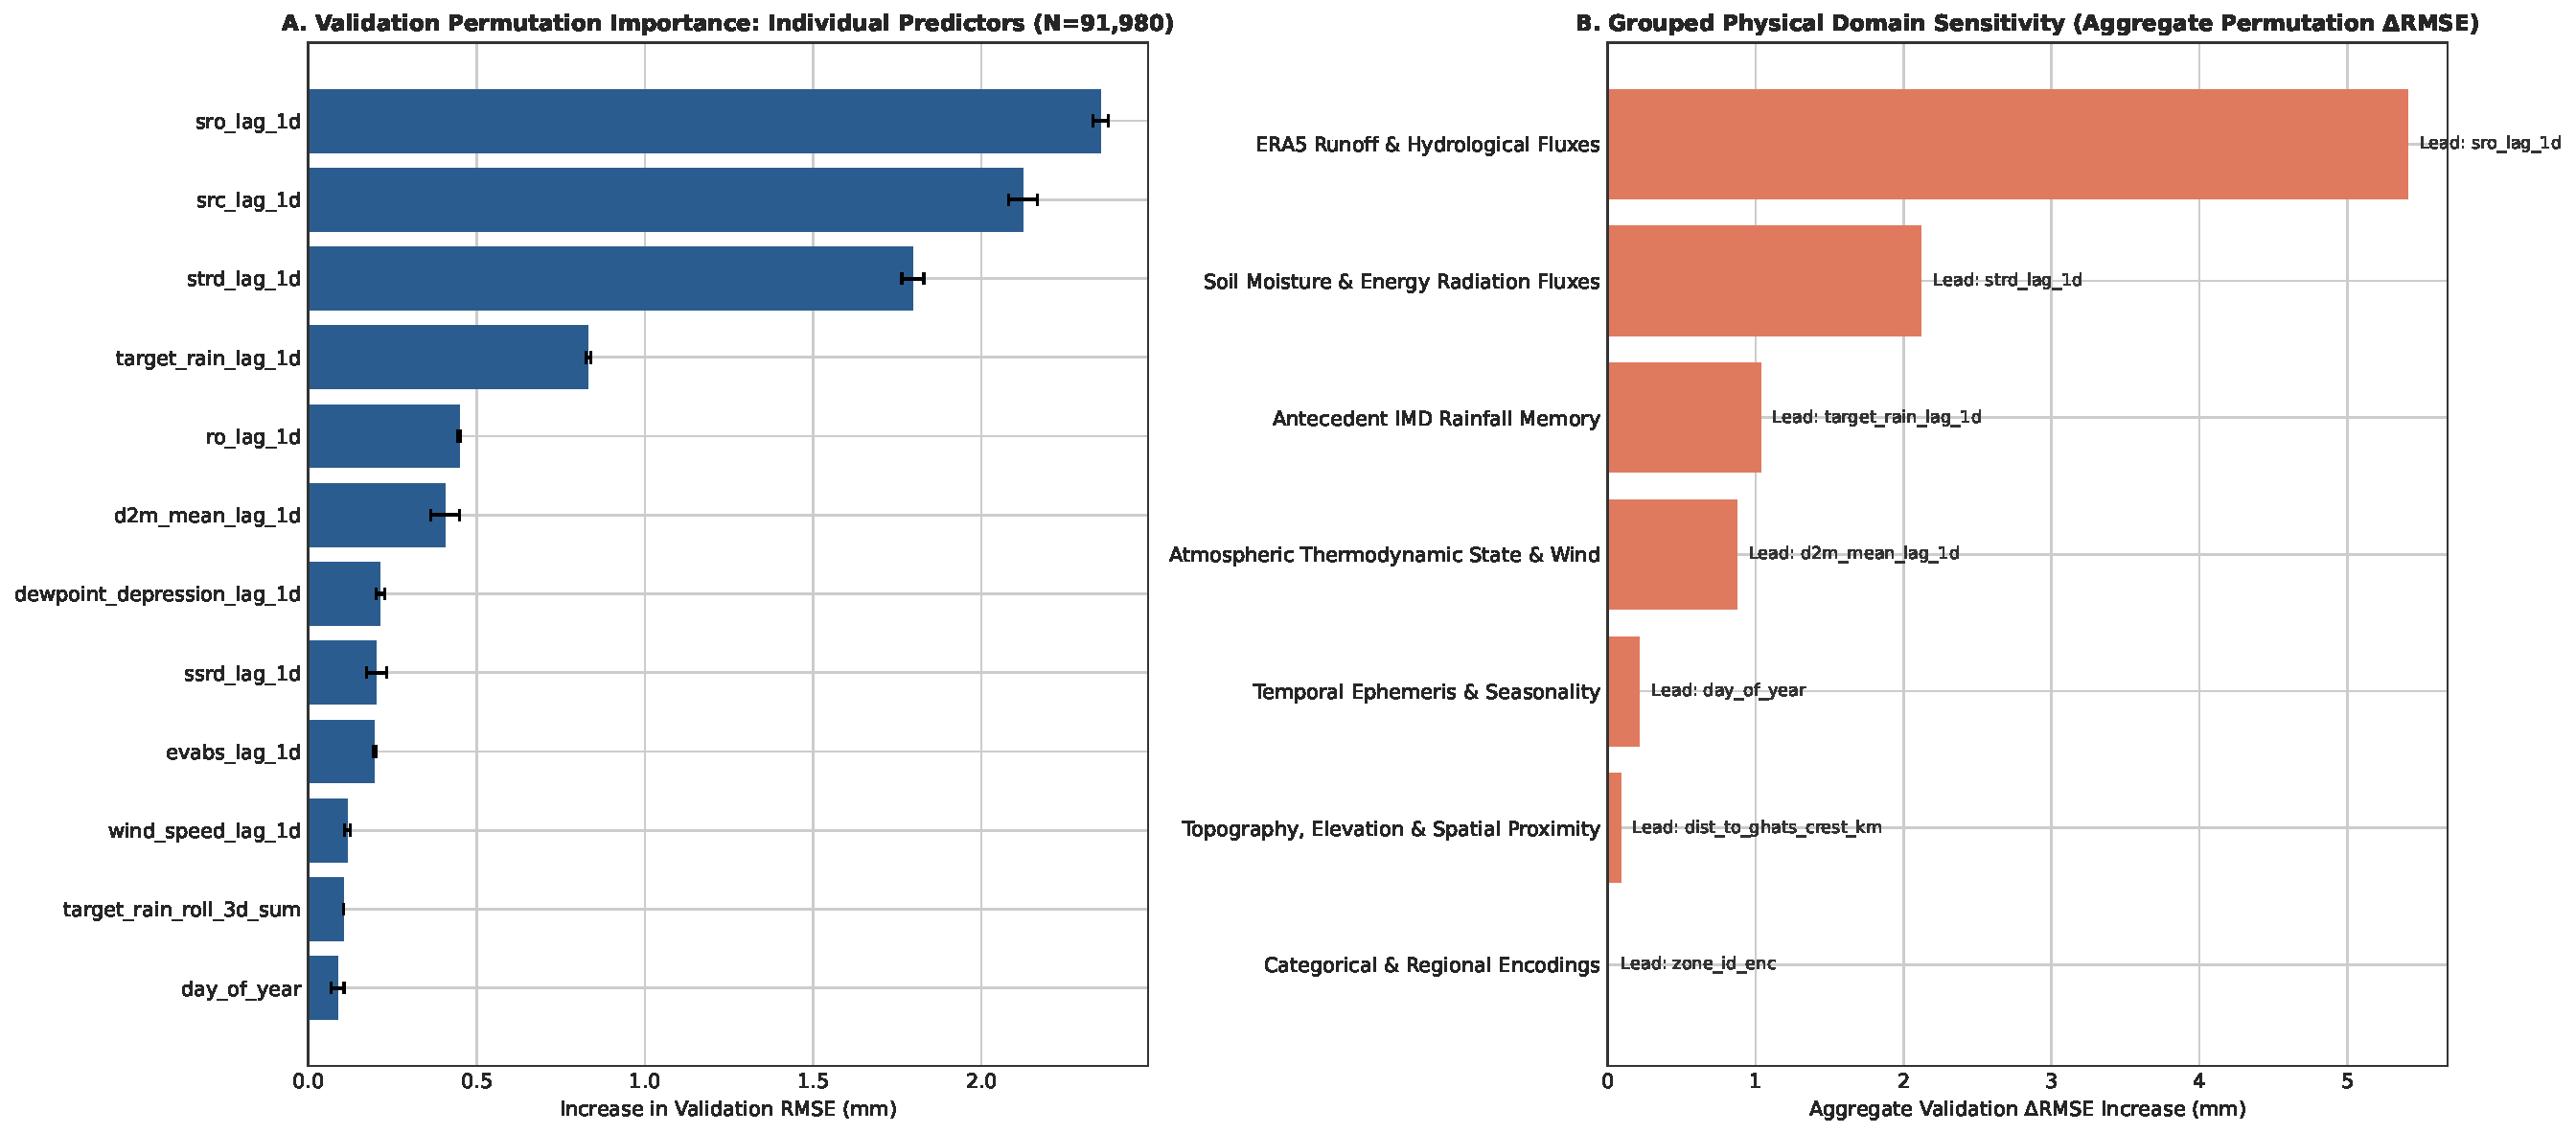
\includegraphics[width=0.85\textwidth]{figures/figure6_feature_interpretation}
\caption{Feature attribution analysis. Panel A shows top 15 predictors ranked by validation permutation RMSE degradation; Panel B shows relative gain contribution by physical predictor domain.}
\label{fig:attribution}
\end{figure}

\begin{table*}[htbp]
\centering
\caption{Systematic Feature Ablation Matrix (Validation 2023 and Test 2024--2025)}
\label{tab:ablation}
\resizebox{\textwidth}{!}{
\begin{tabular}{llcr r r r r r r p{4.5cm}}
\toprule
\textbf{Scenario ID} & \textbf{Ablation Description} & \textbf{Features Retained Count} & \textbf{Validation RMSE mm} & \textbf{Validation KGE 2012} & \textbf{Validation Heavy CSI} & \textbf{Test RMSE mm} & \textbf{Test KGE 2012} & \textbf{Test Heavy CSI} & \textbf{$\Delta$ Test RMSE vs Full mm} & \textbf{Scientific Interpretation} \\
\midrule
Scenario A & A All 63 Primary Predictors & 63 & 5.585 & 0.6494 & 0.4098 & 7.4427 & 0.6245 & 0.2868 & 0.0 & Champion full configuration \\
Scenario B & B Without Runoff and Hydrological Fluxes & 55 & 5.7149 & 0.6463 & 0.4129 & 7.6854 & 0.5925 & 0.2721 & 0.2427 & Hydrological land fluxes provide critical moisture saturation proxies \\
Scenario C & C Without Antecedent IMD Rainfall & 51 & 5.7147 & 0.6235 & 0.3316 & 7.5828 & 0.607 & 0.2693 & 0.1401 & Local gauge memory essential for extreme threshold alerting \\
Scenario D & D Without Terrain and Spatial Predictors & 55 & 5.5809 & 0.6479 & 0.4097 & 7.4557 & 0.6252 & 0.2843 & 0.013 & Terrain captures spatial orographic boundaries \\
Scenario E & E Without ERA5 Predictors & 26 & 6.3909 & 0.4181 & 0.2652 & 8.4511 & 0.4833 & 0.1536 & 1.0084 & ERA5 atmospheric predictors provide measurable incremental predictive value \\
Scenario F & F Only Antecedent IMD and Temporal & 18 & 6.4289 & 0.4193 & 0.3043 & 8.5145 & 0.4686 & 0.1456 & 1.0718 & Baseline autoregressive floor \\
\bottomrule
\end{tabular}
}
\end{table*}

In the LightGBM Focal Loss heavy rainfall classifier, sub-surface runoff (\texttt{ro\_lag\_1d}, $28.11\%$) and surface runoff (\texttt{sro\_lag\_1d}, $26.41\%$) together account for $54.52\%$ of total tree split gain. In continuous LightGBM Tweedie regression, surface runoff accounts for $34.61\%$ of tree gain and skin reservoir content accounts for $28.28\%$. In validation permutation importance ($N = 91,980$, 3 random seeds), surface runoff ranks first ($+2.3545$\;mm RMSE degradation, $+42.16\%$ increase), followed by skin reservoir content ($+2.1241$\;mm) and downward longwave flux ($+1.7960$\;mm). Ablation Scenario E confirms that excluding ERA5-Land predictors degrades Test RMSE from $7.4427$\;mm to $8.4511$\;mm ($+1.0084$\;mm), demonstrating their measurable incremental predictive value beyond local gauge autoregression.

\subsection{Regional and Seasonal Disaggregation}
Table~\ref{tab:regional} and Figure~\ref{fig:regional} detail model performance across Karnataka's four meteorological subdivisions and four climatological seasons.

\begin{table*}[htbp]
\centering
\caption{Subdivisional and Seasonal Stratified Performance on Test Partition}
\label{tab:regional}
\resizebox{\textwidth}{!}{
\begin{tabular}{lllr r r r r r r r r}
\toprule
\textbf{Stratum Type} & \textbf{Stratum Name} & \textbf{Sample Count} & \textbf{Observed Mean mm} & \textbf{ML RMSE mm} & \textbf{Persistence RMSE mm} & \textbf{Raw ERA5 RMSE mm} & \textbf{ML Mean Bias mm} & \textbf{ML PBias pct} & \textbf{ML Pearson r} & \textbf{ML KGE 2012} & \textbf{ML Heavy CSI 64.5mm} \\
\midrule
Meteorological Subdivision & Coastal Karnataka All 13 cells & 9503 & 13.1855 & 14.9475 & 20.3843 & 19.3674 & -1.3244 & -10.04 & 0.8261 & 0.7407 & 0.362 \\
Meteorological Subdivision & Malnad 35 cells & 25585 & 6.3706 & 9.3018 & 12.7091 & 13.2843 & 0.1661 & 2.61 & 0.8043 & 0.7256 & 0.3441 \\
Meteorological Subdivision & North Interior Karnataka 118 cells & 86258 & 2.3758 & 6.4317 & 9.0913 & 9.5698 & 0.0196 & 0.83 & 0.5274 & 0.3676 & 0.0296 \\
Meteorological Subdivision & South Interior Karnataka 86 cells & 62866 & 2.4364 & 6.0472 & 8.5112 & 8.1312 & 0.0531 & 2.18 & 0.5513 & 0.3723 & 0.0 \\
Meteorological Subdivision & Coastal Fallback Only 3 cells IDs 52 68 125 & 2193 & 13.8286 & 15.5086 & 21.61 & 20.3891 & -0.8294 & -6.0 & 0.828 & 0.7504 & 0.3898 \\
Meteorological Subdivision & Coastal Native Land Only 10 cells & 7310 & 12.9925 & 14.7751 & 20.0019 & 19.0503 & -1.4729 & -11.34 & 0.8258 & 0.7356 & 0.3516 \\
Seasonal Regime & Southwest Monsoon JJAS & 61488 & 7.0215 & 10.1883 & 14.1842 & 14.9381 & 0.1431 & 2.04 & 0.7545 & 0.6451 & 0.3355 \\
Seasonal Regime & Post Monsoon Northeast OND & 46368 & 2.1379 & 6.1093 & 8.829 & 7.9161 & 0.0612 & 2.86 & 0.5628 & 0.3823 & 0.0 \\
Seasonal Regime & Pre Monsoon MAM & 46368 & 2.4463 & 6.6839 & 8.9736 & 8.6417 & -0.3207 & -13.11 & 0.6717 & 0.4859 & 0.093 \\
Seasonal Regime & Winter JF & 29988 & 0.0698 & 0.806 & 1.2303 & 1.2443 & -0.0023 & -3.3 & 0.4881 & 0.3436 & 0.0 \\
\bottomrule
\end{tabular}
}
\end{table*}

\begin{figure}[htbp]
\centering
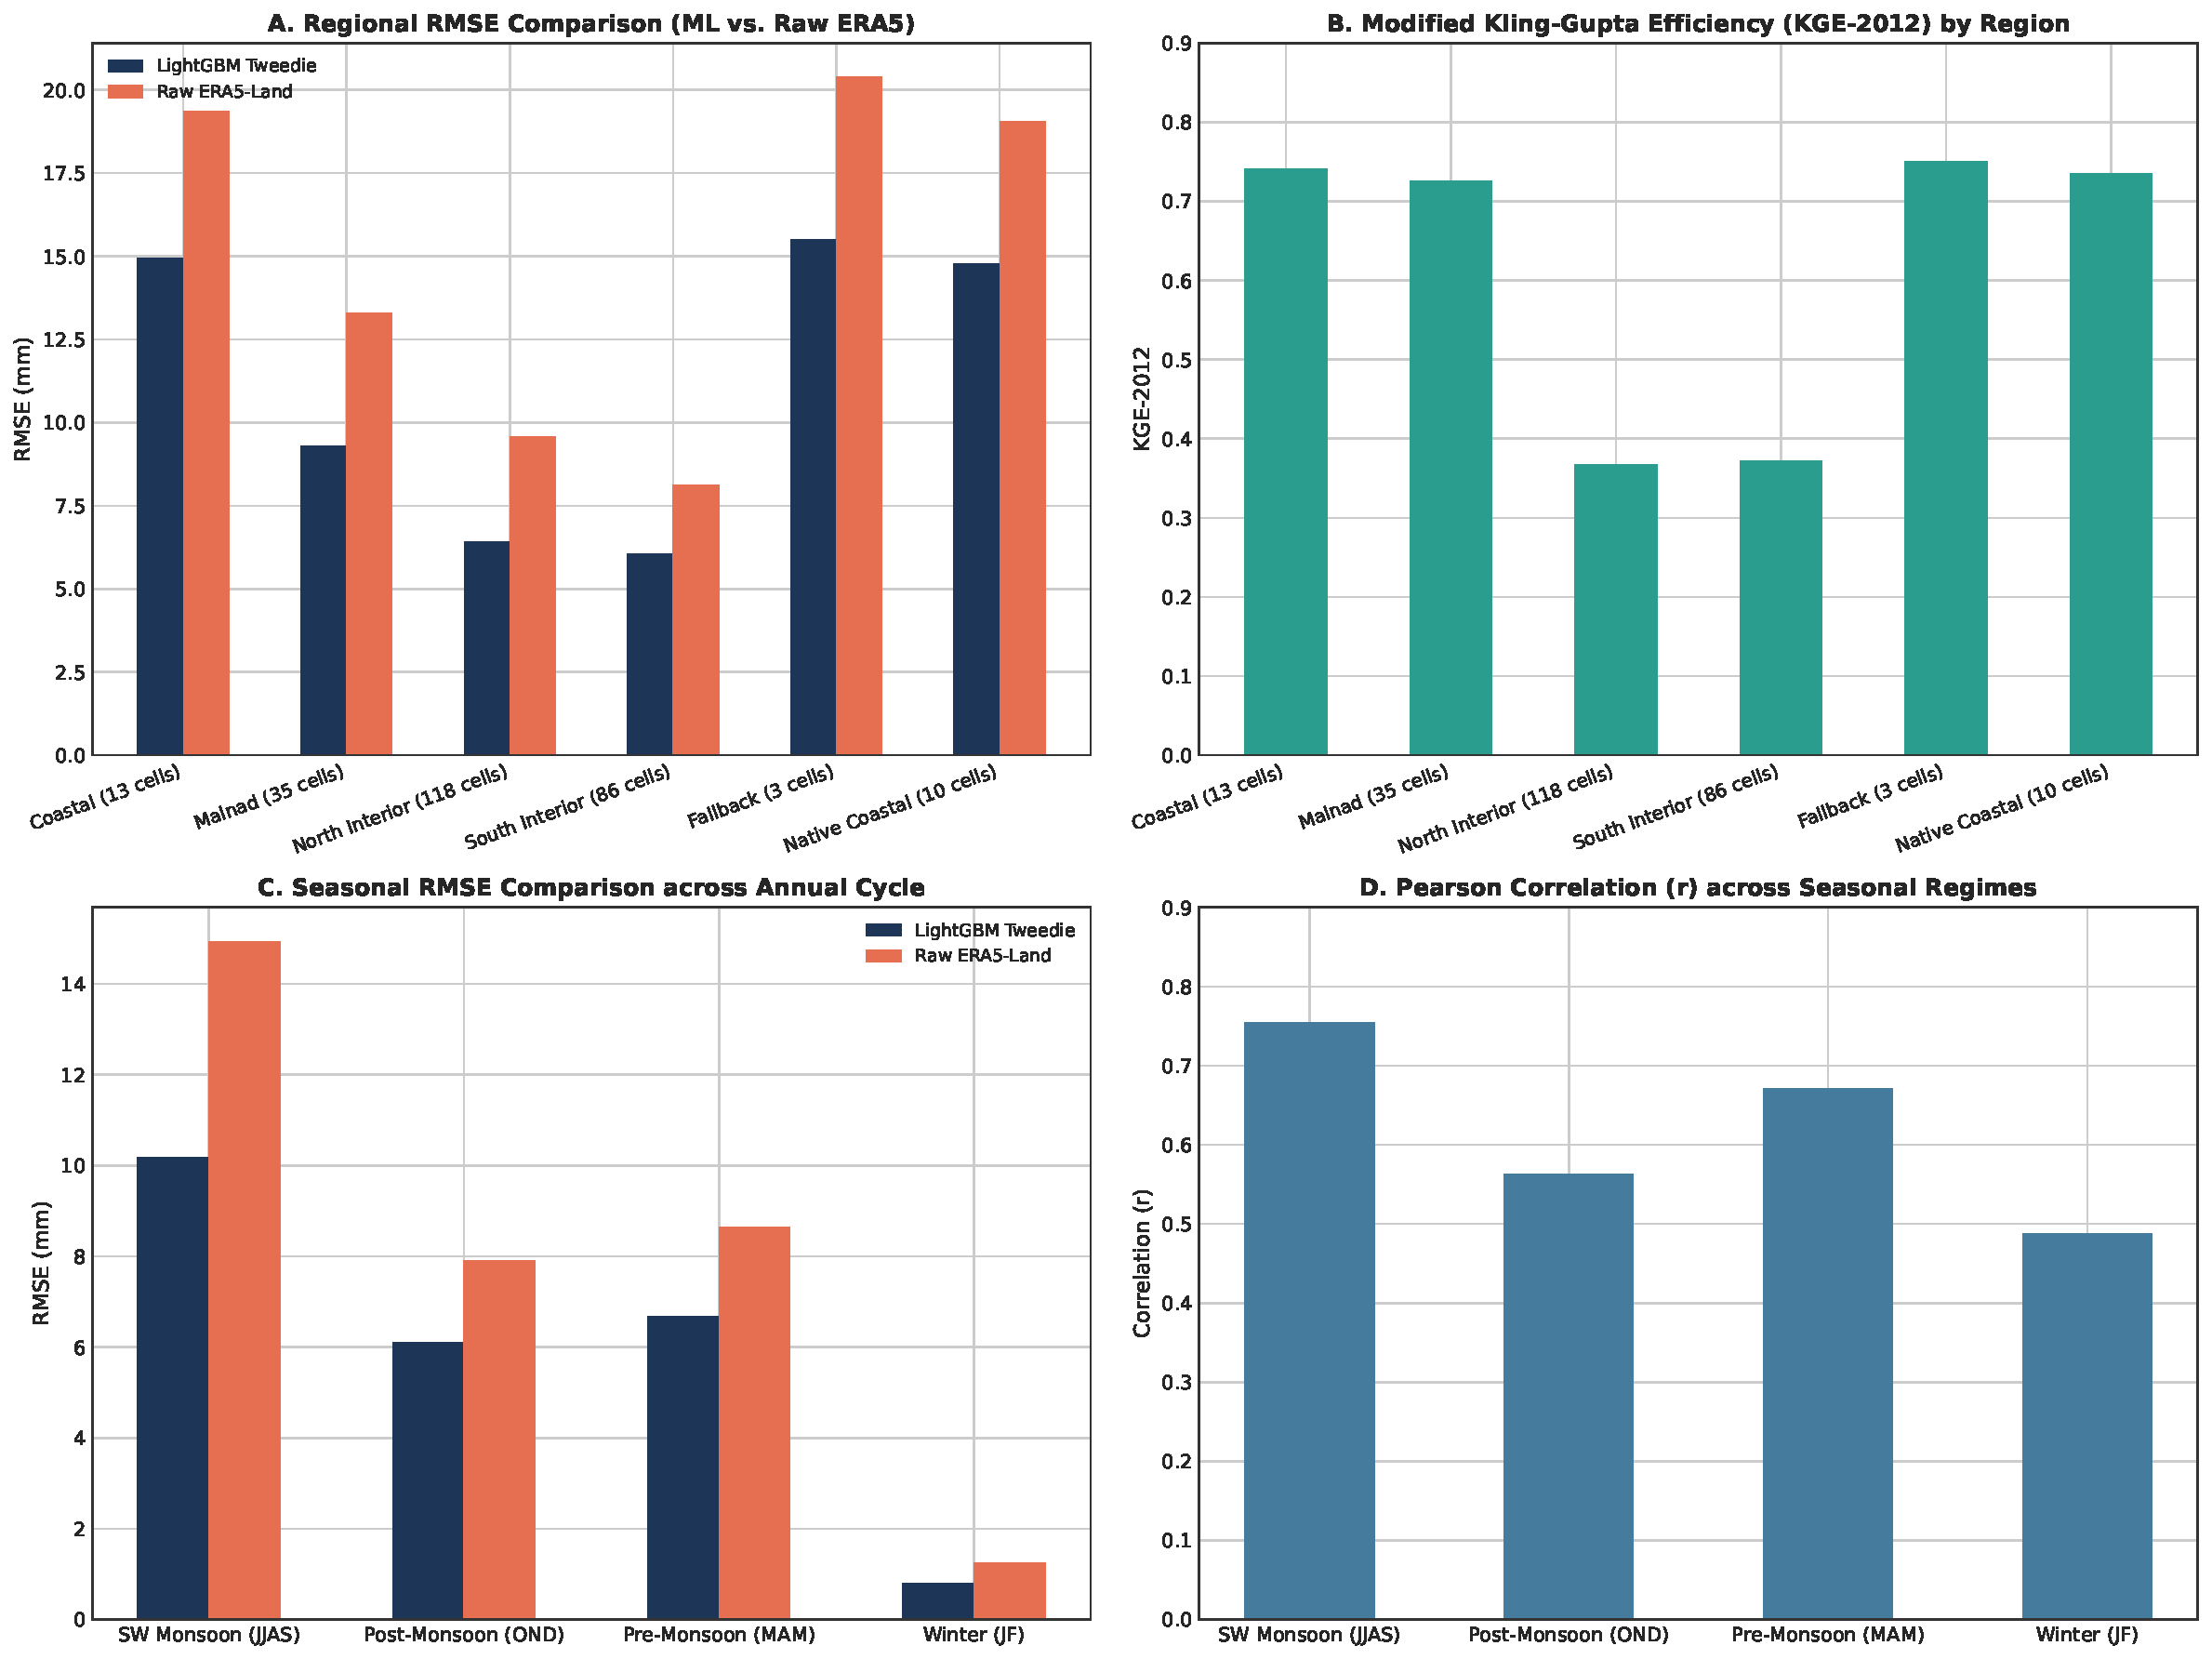
\includegraphics[width=0.88\textwidth]{figures/figure7_regional_seasonal}
\caption{Subdivisional and seasonal hydrometeorological stratification. Panel A shows RMSE and KGE-2012 across subdivisions; Panel B shows seasonal progression across Southwest Monsoon, Post-Monsoon, Pre-Monsoon, and Winter.}
\label{fig:regional}
\end{figure}

In orographic Coastal Karnataka and Malnad, the model achieves high correlation ($r = 0.80$--$0.83$) and hydrological skill ($\text{KGE-2012} = 0.73$--$0.74$). Over the semi-arid interior plains (NIK and SIK), correlation encounters a distinct ceiling ($r \sim 0.53$--$0.55$; $\text{KGE} \sim 0.37$). The 3 coastal fallback cells (Grid-Cell IDs 52, 68, 125; $N = 2,193$) achieve $\text{RMSE} = 15.51$\;mm and $\text{KGE} = 0.7504$, tracking closely with the 10 native-land coastal cells ($\text{RMSE} = 14.78$\;mm, $\text{KGE} = 0.7356$), confirming that nearest-inland neighbor extraction effectively preserves the orographic moisture advection signal.

\subsection{Temporal Generalisation Across Forward Evaluation Years \& Block Bootstrap}
To evaluate out-of-sample temporal generalisation, model performance was audited separately for the two held-out forward calendar years in Table~\ref{tab:annual}. In 2024 ($N = 92,232$; active monsoon convective year), LightGBM Tweedie achieved $\text{RMSE} = 7.5094$\;mm, $\text{MAE} = 3.0074$\;mm, $\text{Bias} = +0.3442$\;mm ($+10.26\%$), $r = 0.7320$, $\text{NSE} = 0.5346$, and $\text{KGE-2012} = 0.5676$. In 2025 ($N = 91,980$; subdued monsoon year), LightGBM Tweedie achieved $\text{RMSE} = 7.3752$\;mm, $\text{MAE} = 2.7909$\;mm, $\text{Bias} = -0.3810$\;mm ($-10.40\%$), $r = 0.7426$, $\text{NSE} = 0.5493$, and $\text{KGE-2012} = 0.6541$. CatBoost Tweedie achieved RMSE of $7.5253$\;mm in 2024 and $7.3403$\;mm in 2025; Hurdle Expected Value achieved RMSE of $7.5210$\;mm in 2024 and $7.3257$\;mm in 2025.

\begin{table*}[htbp]
\centering
\caption{Annual Out-of-Sample Performance Breakdown: 2024 (Leap Year) vs. 2025}
\label{tab:annual}
\resizebox{\textwidth}{!}{
\begin{tabular}{llr r r r r r r r r r}
\toprule
\textbf{Strata} & \textbf{Model} & \textbf{N} & \textbf{Obs Mean} & \textbf{Pred Mean} & \textbf{MAE mm} & \textbf{RMSE mm} & \textbf{Bias mm} & \textbf{PBias pct} & \textbf{Pearson r} & \textbf{NSE} & \textbf{KGE 2012} \\
\midrule
Year\_2024\_Full & LightGBM\_Tweedie & 92232 & 3.3539 & 3.6981 & 3.0074 & 7.5094 & 0.3442 & 10.26 & 0.732 & 0.5346 & 0.5676 \\
Year\_2024\_Full & CatBoost\_Tweedie & 92232 & 3.3539 & 3.7431 & 3.0289 & 7.5253 & 0.3892 & 11.6 & 0.7309 & 0.5327 & 0.5577 \\
Year\_2024\_Full & Hurdle\_ExpectedValue & 92232 & 3.3539 & 3.7534 & 3.05 & 7.521 & 0.3995 & 11.91 & 0.7311 & 0.5332 & 0.5436 \\
Year\_2024\_Full & Persistence & 92232 & 3.3539 & 3.3539 & 3.6498 & 10.3927 & -0.0 & -0.0 & 0.5543 & 0.1087 & 0.5543 \\
Year\_2024\_Full & Raw\_ERA5 & 92232 & 3.3539 & 4.1579 & 4.1904 & 10.6003 & 0.8041 & 23.97 & 0.4789 & 0.0727 & 0.3527 \\
Year\_2024\_Full & EQM & 92232 & 3.3539 & 3.9681 & 4.2069 & 11.1297 & 0.6142 & 18.31 & 0.493 & -0.0222 & 0.4403 \\
Year\_2025\_Full & LightGBM\_Tweedie & 91980 & 3.6644 & 3.2834 & 2.7909 & 7.3752 & -0.381 & -10.4 & 0.7426 & 0.5493 & 0.6541 \\
Year\_2025\_Full & CatBoost\_Tweedie & 91980 & 3.6644 & 3.3519 & 2.808 & 7.3403 & -0.3125 & -8.53 & 0.7446 & 0.5535 & 0.6689 \\
Year\_2025\_Full & Hurdle\_ExpectedValue & 91980 & 3.6644 & 3.3324 & 2.8096 & 7.3257 & -0.332 & -9.06 & 0.7466 & 0.5553 & 0.6538 \\
Year\_2025\_Full & Persistence & 91980 & 3.6644 & 3.6644 & 3.8522 & 10.3236 & 0.0 & 0.0 & 0.5584 & 0.1168 & 0.5584 \\
Year\_2025\_Full & Raw\_ERA5 & 91980 & 3.6644 & 3.9717 & 4.0926 & 10.3073 & 0.3073 & 8.39 & 0.5038 & 0.1196 & 0.4592 \\
Year\_2025\_Full & EQM & 91980 & 3.6644 & 3.823 & 4.2165 & 11.264 & 0.1586 & 4.33 & 0.4957 & -0.0514 & 0.4938 \\
\bottomrule
\end{tabular}
}
\end{table*}

\begin{table*}[htbp]
\centering
\caption{Stationary Block Bootstrap Statistical Significance (2,000 Replicates on Test Partition)}
\label{tab:bootstrap}
\resizebox{\textwidth}{!}{
\begin{tabular}{llp{4.5cm}r r r r r c c}
\toprule
\textbf{Model Pair} & \textbf{Block Length Days} & \textbf{Temporal Memory Assumption} & \textbf{Bootstrap Replicates} & \textbf{Mean $\Delta$ RMSE mm} & \textbf{Standard Error mm} & \textbf{CI 95 Low mm} & \textbf{CI 95 High mm} & \textbf{Replicates $\Delta$ ge Zero} & \textbf{Empirical p Value Resolution} \\
\midrule
LightGBM\_Tweedie vs. Persistence & 7 & Synoptic weather persistence (7d) & 2000 & -2.925 & 0.2046 & -3.3241 & -2.5175 & 0 & p $<$ 0.0005 \\
LightGBM\_Tweedie vs. EQM & 7 & Synoptic weather persistence (7d) & 2000 & -3.7542 & 0.3768 & -4.4626 & -3.0039 & 0 & p $<$ 0.0005 \\
LightGBM\_Tweedie vs. Raw\_ERA5 & 7 & Synoptic weather persistence (7d) & 2000 & -3.0109 & 0.3482 & -3.7037 & -2.3735 & 0 & p $<$ 0.0005 \\
CatBoost\_Tweedie vs. Persistence & 7 & Synoptic weather persistence (7d) & 2000 & -2.9337 & 0.2077 & -3.3415 & -2.5276 & 0 & p $<$ 0.0005 \\
CatBoost\_Tweedie vs. EQM & 7 & Synoptic weather persistence (7d) & 2000 & -3.7629 & 0.3848 & -4.4936 & -2.9954 & 0 & p $<$ 0.0005 \\
Hurdle\_ExpectedValue vs. Persistence & 7 & Synoptic weather persistence (7d) & 2000 & -2.9436 & 0.2025 & -3.3413 & -2.5449 & 0 & p $<$ 0.0005 \\
Hurdle\_ExpectedValue vs. EQM & 7 & Synoptic weather persistence (7d) & 2000 & -3.7728 & 0.3824 & -4.4955 & -3.0224 & 0 & p $<$ 0.0005 \\
LightGBM\_Tweedie vs. Persistence & 14 & Bi-weekly intraseasonal / MJO persistence (14d) & 2000 & -2.9298 & 0.2271 & -3.3608 & -2.4729 & 0 & p $<$ 0.0005 \\
LightGBM\_Tweedie vs. EQM & 14 & Bi-weekly intraseasonal / MJO persistence (14d) & 2000 & -3.7645 & 0.4243 & -4.5976 & -2.9587 & 0 & p $<$ 0.0005 \\
LightGBM\_Tweedie vs. Raw\_ERA5 & 14 & Bi-weekly intraseasonal / MJO persistence (14d) & 2000 & -3.0204 & 0.3785 & -3.7669 & -2.3255 & 0 & p $<$ 0.0005 \\
CatBoost\_Tweedie vs. Persistence & 14 & Bi-weekly intraseasonal / MJO persistence (14d) & 2000 & -2.9382 & 0.2322 & -3.38 & -2.4688 & 0 & p $<$ 0.0005 \\
CatBoost\_Tweedie vs. EQM & 14 & Bi-weekly intraseasonal / MJO persistence (14d) & 2000 & -3.7729 & 0.4338 & -4.6235 & -2.955 & 0 & p $<$ 0.0005 \\
Hurdle\_ExpectedValue vs. Persistence & 14 & Bi-weekly intraseasonal / MJO persistence (14d) & 2000 & -2.948 & 0.2293 & -3.3901 & -2.4876 & 0 & p $<$ 0.0005 \\
Hurdle\_ExpectedValue vs. EQM & 14 & Bi-weekly intraseasonal / MJO persistence (14d) & 2000 & -3.7827 & 0.4309 & -4.6238 & -2.963 & 0 & p $<$ 0.0005 \\
\bottomrule
\end{tabular}
}
\end{table*}

\begin{figure}[htbp]
\centering
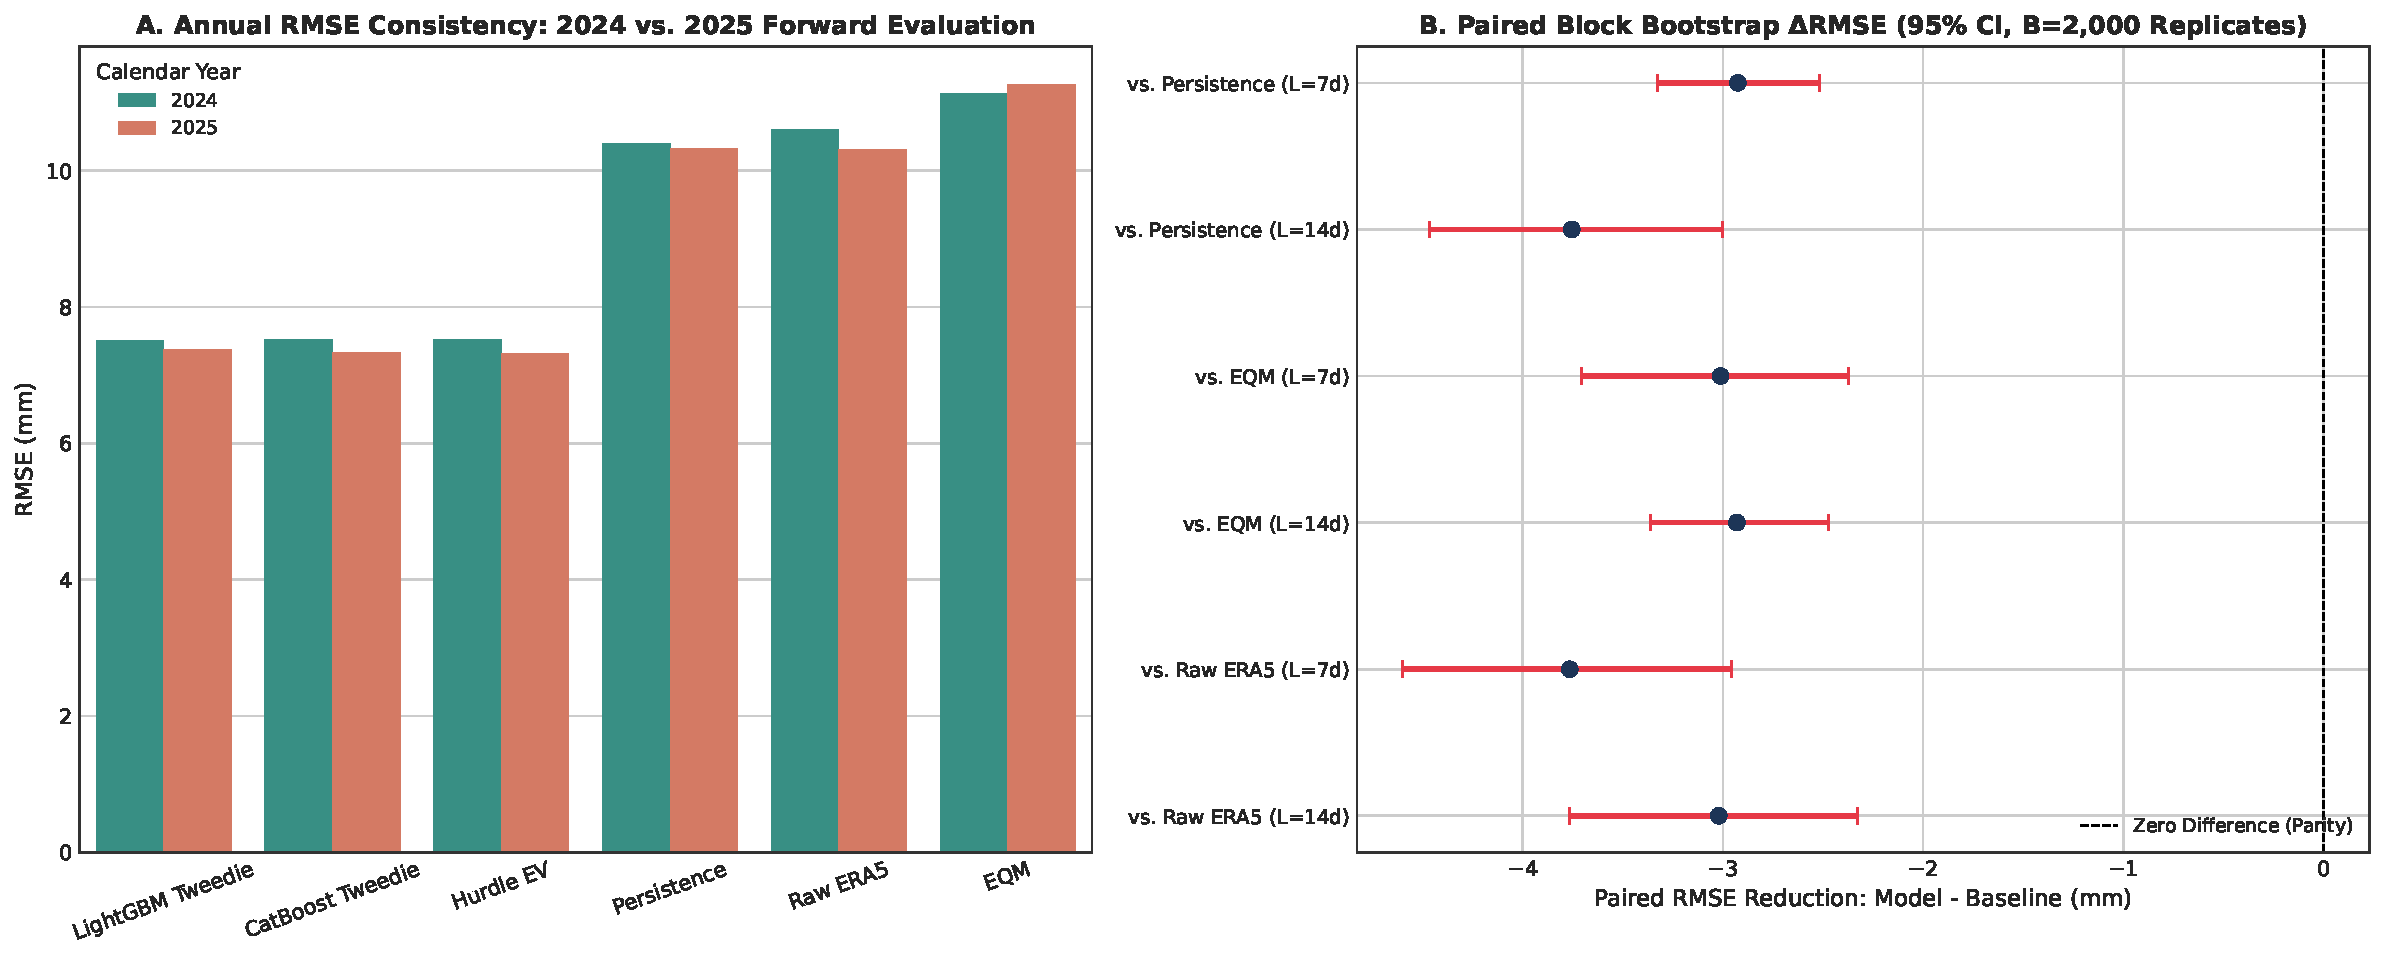
\includegraphics[width=0.88\textwidth]{figures/figure8_temporal_robustness}
\caption{Temporal robustness and block bootstrap confidence intervals. Panel A shows annual RMSE consistency bar comparison across 2024 and 2025 forward evaluation years; Panel B shows paired block bootstrap 95\% confidence interval error bars ($B = 2,000$ replicates, empirical resolution $p < 0.0005$) for $L=7\text{d}$ and $L=14\text{d}$ block lengths.}
\label{fig:robustness}
\end{figure}

Across all 2,000 block bootstrap resamples under both 7-day and 14-day block lengths (Table~\ref{tab:bootstrap} and Fig.~\ref{fig:robustness}), zero replicates yielded $\Delta \text{RMSE} \ge 0$, establishing that the paired stationary block-bootstrap analysis provides strong statistical evidence of lower RMSE under the evaluated resampling assumptions (empirical resolution $p < 0.0005$).

\subsection{Rainfall Intensity Limitations \& Extreme Quantile Shrinkage}
Table~\ref{tab:intensity} and Figure~\ref{fig:extremes} provide an audit of continuous model behavior across the seven official IMD rainfall intensity categories.

\begin{table*}[htbp]
\centering
\caption{Rainfall Intensity Error Profiles and Extreme Quantile Shrinkage (Test Set; $N = 184,212$)}
\label{tab:intensity}
\resizebox{\textwidth}{!}{
\begin{tabular}{lr r r r r r r r r r r p{4cm}}
\toprule
\textbf{IMD Rainfall Intensity Category} & \textbf{Sample Count} & \textbf{Percent Total Test Data} & \textbf{Observed Mean mm} & \textbf{Observed Std mm} & \textbf{Predicted Mean mm} & \textbf{Predicted Std mm} & \textbf{MAE mm} & \textbf{RMSE mm} & \textbf{Mean Bias mm} & \textbf{Percentage Bias pct} & \textbf{Percent Underestimated} & \textbf{Structural Limitation Note} \\
\midrule
No Rain ($<$0.1 mm) & 119669 & 64.96 & 0.0 & 0.0 & 0.77 & 1.96 & 0.77 & 2.1 & 0.77 & Undefined\textsuperscript{*} & 0.0 & Near-zero background drizzle inflation \\
Very Light (0.1--2.4 mm) & 26590 & 14.43 & 0.96 & 0.69 & 4.04 & 4.04 & 3.29 & 5.05 & 3.08 & 319.1 & 16.9 & Overestimation due to exponential link penalty \\
Light (2.5--15.5 mm) & 25854 & 14.03 & 7.03 & 3.6 & 7.46 & 6.53 & 4.67 & 6.58 & 0.43 & 6.1 & 53.8 & Optimal continuous calibration sweet spot \\
Moderate (15.6--64.4 mm) & 10832 & 5.88 & 29.81 & 12.29 & 17.22 & 15.23 & 16.55 & 20.21 & -12.59 & -42.2 & 83.5 & Progressive underestimation onset \\
Heavy (64.5--115.5 mm) & 1067 & 0.58 & 81.68 & 13.12 & 46.98 & 28.89 & 37.58 & 44.39 & -34.71 & -42.5 & 88.6 & Severe extreme quantile shrinkage (conditional expectation cap) \\
Very Heavy (115.6--204.4 mm) & 192 & 0.1 & 141.52 & 20.68 & 71.53 & 27.63 & 70.0 & 77.72 & -70.0 & -49.5 & 100.0 & Severe extreme quantile shrinkage (conditional expectation cap) \\
Extremely Heavy ($\ge$204.5 mm) & 8 & 0.0043 & 225.02 & 18.7 & 73.66 & 27.99 & 151.36 & 154.76 & -151.36 & -67.3 & 100.0 & Severe extreme quantile shrinkage (conditional expectation cap) \\
\bottomrule
\end{tabular}
}
\end{table*}

\begin{figure}[htbp]
\centering
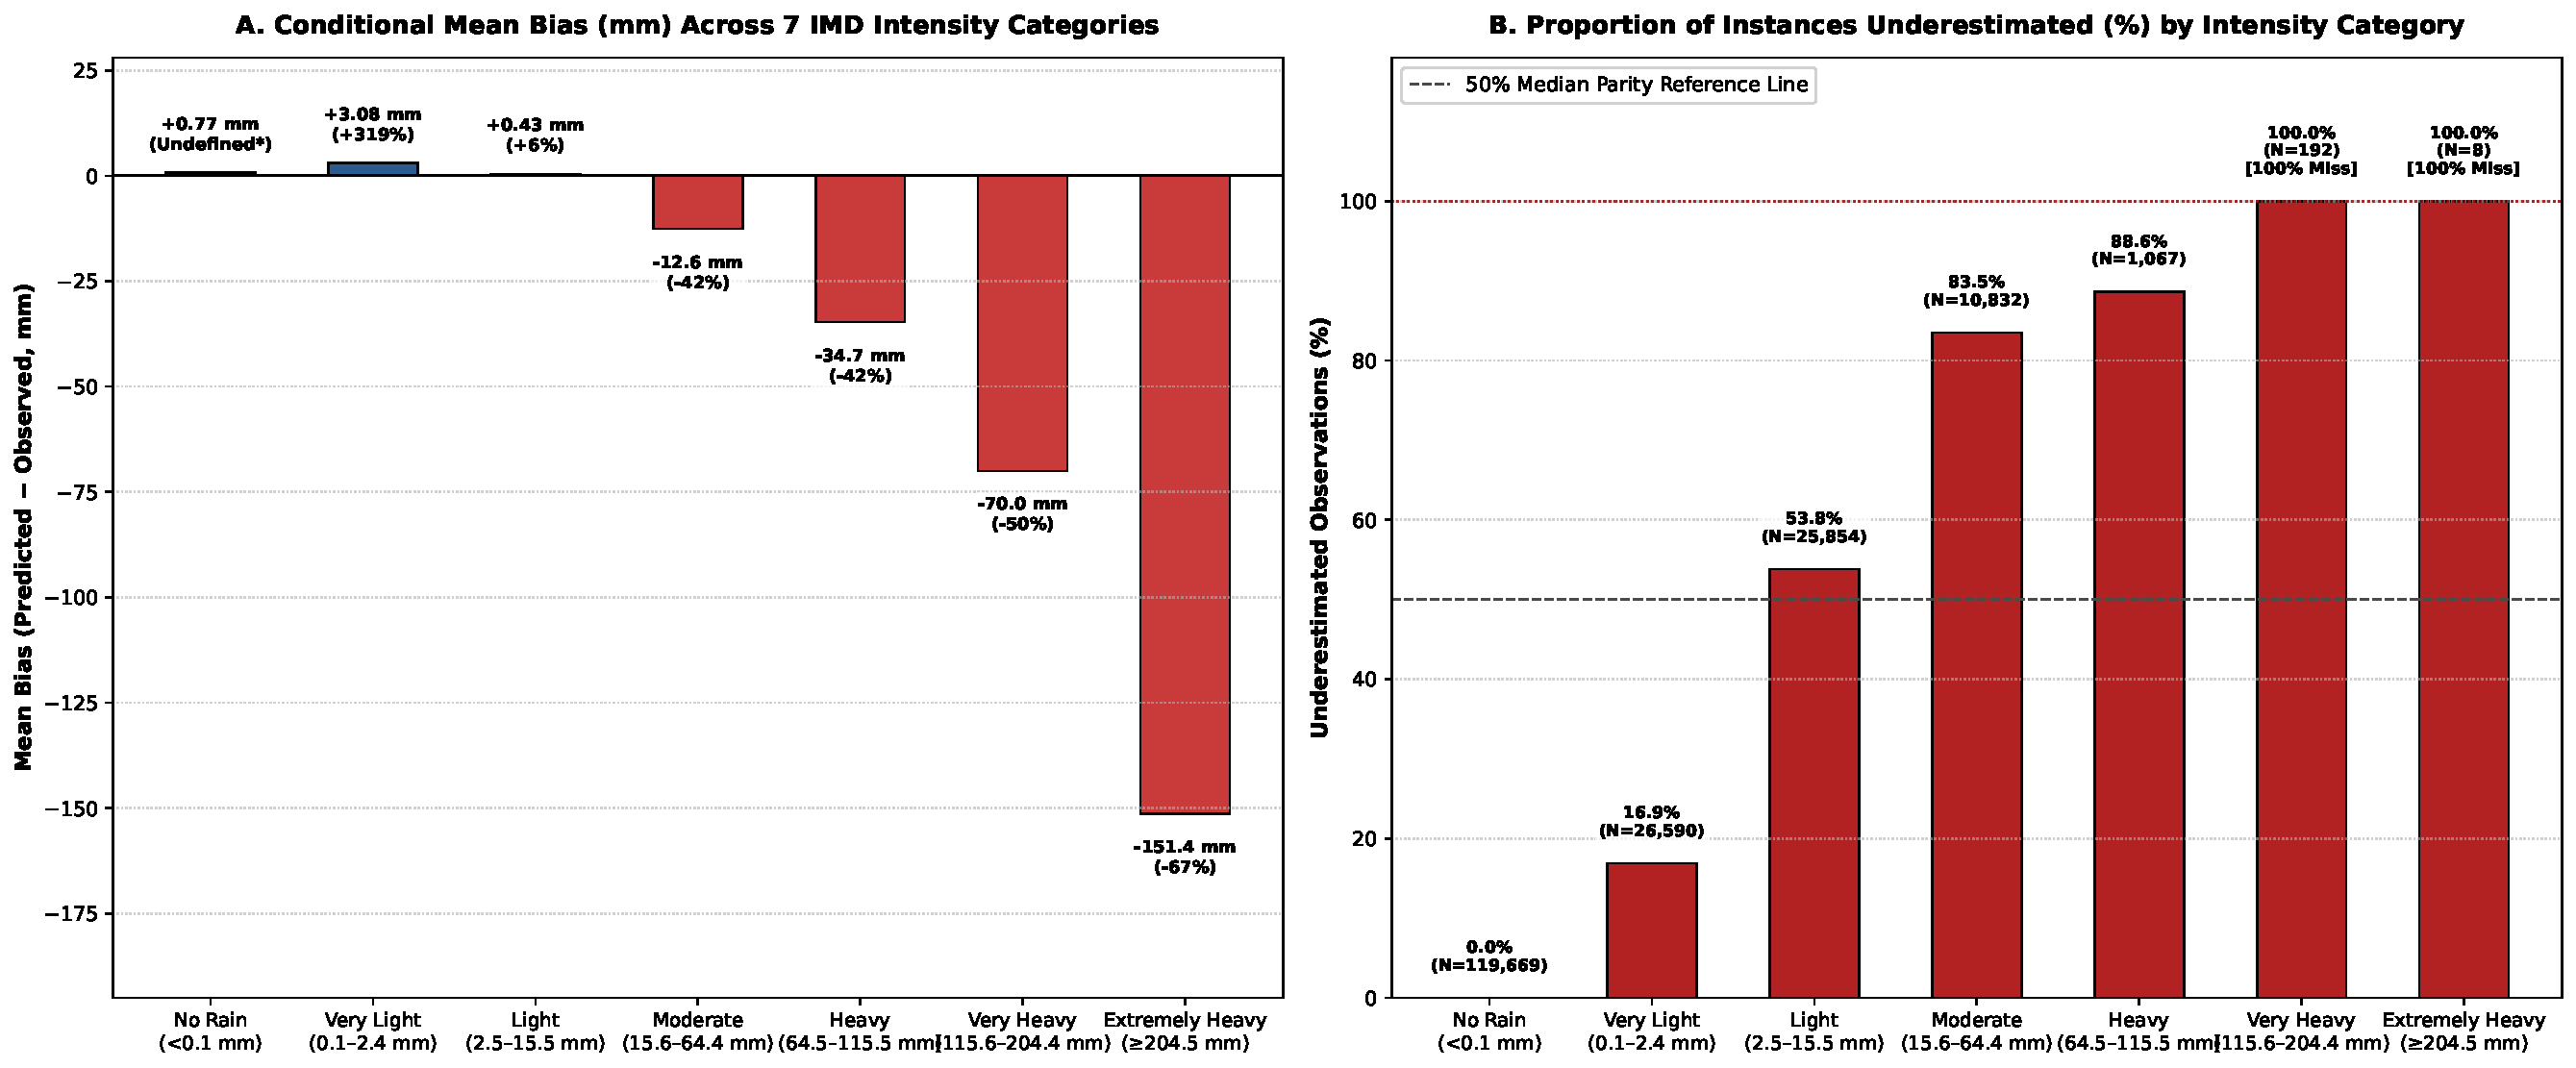
\includegraphics[width=0.88\textwidth]{figures/figure9_extreme_rainfall_errors}
\caption{Rainfall intensity error profiles and quantile shrinkage. Panel A shows Mean Bias (mm) and Percentage Bias (\%) across the 7 IMD categories; Panel B shows underestimation frequency (\%) and sample counts.}
\label{fig:extremes}
\end{figure}

A critical structural limitation is documented: continuous conditional expectation models underestimate $100.0\%$ of test observations exceeding $115.6$\;mm ($200$ events, comprising 192 Very Heavy and 8 Extremely Heavy events), with predictions plateauing near $70$--$90$\;mm despite observed extremes up to $286.0$\;mm. Furthermore, on true dry days ($<0.1$\;mm; $N = 119,669$; $64.96\%$ of test records), the model exhibits background drizzle inflation ($+0.77$\;mm mean bias; Percentage Bias is undefined due to zero denominator). These structural boundaries prove that continuous regression alone cannot capture localized convective bursts.

\section{Discussion}\label{sec5}

\subsection{Hydrological Memory: Surface Runoff as Soil Saturation Proxy}
A primary physical finding is that land-surface runoff fluxes account for $54.52\%$ of total tree gain in heavy rain classification and lead permutation importance in continuous regression. Crucially, ERA5-Land runoff variables represent simulated land-surface water fluxes from ECMWF's HTESSEL land model, rather than direct streamflow observations. In tropical monsoonal regimes, modeled surface runoff is generated only when local infiltration capacity is exceeded or topsoil approaches saturation. Runoff fluxes act as a physical integrator, filtering out transient atmospheric false alarms and retaining sustained moisture convergence.

\subsection{The Conditional Mean Ceiling \& Disaster-Risk Alerting Limitations}
The severe underestimation of extreme rainfall ($\ge 115.6$\;mm) is a fundamental mathematical property of conditional mean regression under asymmetric squared-error and deviance loss functions. When extreme events represent $<0.1\%$ of the training distribution, minimizing expected loss pulls predictions toward the conditional mean, truncating the upper tail. For operational hazard warning, continuous models must be decoupled from extreme alerting, or integrated with specialized extreme-value loss formulations.

\subsection{Orographic Trade-offs \& Spatial Bias Dissociation}
The performance dichotomy between orographic Western Ghats ($r \ge 0.80$) and interior Deccan plateau ($r \sim 0.53$) reflects atmospheric scale limits. Western Ghats precipitation is mechanically forced by low-level moisture advection perpendicular to the terrain ridge, which reanalysis resolves with high skill. Conversely, interior precipitation is governed by unorganized, localized mesoscale convective thunderstorm cells unresolvable on a 0.1$^\circ$ grid.

\subsection{Operational Deployment Prerequisites}
Furthermore, we explicitly emphasize that because ERA5-Land has an operational release latency of 2 to 3 months, this framework represents a retrospective hydrometeorological reconstruction and gap-filling pipeline, rather than an operational real-time nowcasting system. The heavy-rain classifier serves as an experimental retrospective classification component ($\text{CSI} = 0.3512$, precision = $58.22\%$), but misses $53.04\%$ of observed heavy events. Operational hazard warning deployment would require extensive forward NWP integration, independent real-time validation, and specialized extreme-event calibration.

\section{Limitations}\label{sec6}
Key structural limitations must be acknowledged:
\begin{enumerate}
    \item \textbf{Retrospective Hindcasting vs. Real-Time Forecasting:} Reanalysis release latency (2--3 months) precludes real-time flood nowcasting.
    \item \textbf{Absence of Spatial Generalisation:} All 252 IMD grid cells were present across partitions; transferability to ungauged basins is untested.
    \item \textbf{Extreme Quantile Shrinkage:} Continuous models underestimate $100.0\%$ of events exceeding $115.6$\;mm ($200$ test events), plateauing at $70$--$90$\;mm.
    \item \textbf{Heavy-Rain Miss Rate \& Unreliable Extreme Alerting:} The focal-loss classifier misses $53.04\%$ of observed heavy events ($\ge 64.5$\;mm) and does not establish reliable detection of very-heavy or extremely-heavy precipitation.
    \item \textbf{Dry-Day Drizzle Inflation:} On true zero-rain days ($N = 119,669$; $64.96\%$ of test records), the continuous model predicts a mean drizzle of $+0.77$\;mm.
    \item \textbf{Frozen Test-Set Access:} Test data was accessed for frozen evaluation and descriptive ablation reporting; zero parameter tuning was performed.
    \item \textbf{Coastal Fallback Strategy:} The 3 coastal margin cells (IDs 52, 68, 125) rely on nearest-inland neighbor extraction due to marine water masking.
    \item \textbf{Predictive Sensitivity vs. Physical Causality:} Feature attribution metrics reflect empirical predictive associations rather than deterministic causal proof.
    \item \textbf{Reanalysis Resolution Limits:} The 0.1$^\circ$ grid spacing cannot resolve meso-gamma convective thunderstorms over interior plains.
\end{enumerate}

\section{Data and Code Availability}\label{sec7}
All modeling workflows, feature extraction scripts, trained model joblib files, and validation routines are available in the project reproducibility package. Gridded daily IMD precipitation data are maintained by the National Data Centre (NDC), India Meteorological Department, Pune (accessible upon user registration). ERA5-Land reanalysis datasets are publicly available from the Copernicus Climate Data Store under an open license.

\section*{Declarations}
\begin{itemize}
    \item \textbf{Funding:} This research received no specific grant from any funding agency in the public, commercial, or not-for-profit sectors.
    \item \textbf{Conflict of Interest:} The authors declare that they have no competing financial or personal interests that could influence the work reported in this paper.
    \item \textbf{Author Contributions:} All authors contributed equally to the study conception, data curation, model development, statistical validation, and manuscript preparation.
\end{itemize}

\begin{thebibliography}{99}

\bibitem{masson2021}
Masson-Delmotte, V., et~al.: IPCC, 2021: Summary for Policymakers. In: Climate Change 2021: The Physical Science Basis. Cambridge University Press, Cambridge (2021)

\bibitem{munoz2021}
Mu{\~n}oz-Sabater, J., et~al.: ERA5-Land: A state-of-the-art global reanalysis dataset for land applications. Earth Syst. Sci. Data 13(9), 4349--4383 (2021). DOI: 10.5194/essd-13-4349-2021

\bibitem{pai2014}
Pai, D.S., et~al.: Development of a new high spatial resolution ($0.25^\circ \times 0.25^\circ$) long period (1901--2010) daily gridded rainfall data set over India and its comparison with existing data sets. Mausam 65(1), 1--18 (2014). DOI: 10.54302/mausam.v65i1.851

\bibitem{rajeevan2006}
Rajeevan, M., Bhate, J., Jaswal, A.K.: Analysis of variability and extremes of daily rainfall over India using a new high resolution gridded data set: 1951--2003. Curr. Sci. 91(3), 296--308 (2006)

\bibitem{copernicus2020}
European Space Agency: Copernicus Global Digital Elevation Model (GLO-90) (2020). DOI: 10.5270/esa-c1qtxnn

\bibitem{goswami2006}
Goswami, B.N., Venugopal, V., Sengupta, D., Madhusoodanan, M.S., Xavier, P.: Increasing trend of extreme rain events over India in a warming environment. Science 314(5804), 1442--1445 (2006). DOI: 10.1126/science.1132027

\bibitem{houze2003}
Houze, R.: Orographic precipitation. Annu. Rev. Earth Planet. Sci. 31, 153--185 (2003). DOI: 10.1146/annurev.earth.31.100901.141251

\bibitem{mohanty2005}
Mohanty, U.C., et~al.: Simulation of heavy precipitation over steep orography of Western Ghats in India using high-resolution mesoscale models. Meteorol. Atmos. Phys. 89, 161--178 (2005). DOI: 10.1007/s00703-005-0167-2

\bibitem{hersbach2020}
Hersbach, H., et~al.: The ERA5 global reanalysis. Q. J. R. Meteorol. Soc. 146(730), 1999--2049 (2020). DOI: 10.1002/qj.3803

\bibitem{piani2011}
Piani, C., et~al.: Statistical bias correction of global simulated daily precipitation and temperature using empirical quantile mapping. J. Climatol. 31(10), 1530--1544 (2011). DOI: 10.1002/joc.2168

\bibitem{cannon2015}
Cannon, A.J., Sobie, S.R., Murdock, T.Q.: Bias correction of GCM precipitation by quantile mapping: How well do methods preserve changes in quantiles and extremes? J. Clim. 28(17), 6938--6959 (2015). DOI: 10.1175/JCLI-D-14-00754.1

\bibitem{bano2020}
Ba{\~n}o-Medina, J., Manzanas, R., Guti{\'e}rrez, J.M.: Configuration and intercomparison of deep learning neural models for statistical downscaling. Geosci. Model Dev. 13(4), 2109--2124 (2020). DOI: 10.5194/gmd-13-2109-2020

\bibitem{reichstein2019}
Reichstein, M., et~al.: Deep learning and process understanding for data-driven Earth system science. Nature 566(7743), 195--204 (2019). DOI: 10.1038/s41586-019-0912-1

\bibitem{ke2017}
Ke, G., et~al.: LightGBM: A highly efficient gradient boosting decision tree. In: Adv. Neural Inf. Process. Syst. (NeurIPS 2017), vol. 30, pp. 3146--3154 (2017)

\bibitem{prokhorenkova2018}
Prokhorenkova, L., Gusev, G., Vorobev, A., Dorogush, A.V., Gulin, A.: CatBoost: unbiased boosting with categorical features. In: Adv. Neural Inf. Process. Syst. (NeurIPS 2018), vol. 31, pp. 6638--6648 (2018)

\bibitem{chen2016}
Chen, T., Guestrin, C.: XGBoost: A scalable tree boosting system. In: Proc. 22nd ACM SIGKDD Int. Conf. Knowl. Discov. Data Min., pp. 785--794 (2016). DOI: 10.1145/2939672.2939785

\bibitem{tweedie1984}
Tweedie, M.C.K.: An index which distinguishes between some important exponential families. In: Statistics: Applications and New Directions, Proc. Indian Stat. Inst. Golden Jubilee Int. Conf., pp. 579--604. Indian Statistical Institute, Calcutta (1984)

\bibitem{dunn2005}
Dunn, P.K., Smyth, G.K.: Series evaluation of Tweedie exponential dispersion model densities. Stat. Comput. 15(4), 267--280 (2005). DOI: 10.1007/s11222-005-4070-y

\bibitem{cragg1971}
Cragg, J.G.: Some statistical models for limited dependent variables with application to the demand for durable goods. Econometrica 39(5), 829--844 (1971). DOI: 10.2307/1909582

\bibitem{duan1983}
Duan, N.: Smearing estimate: A nonparametric retransformation method. J. Am. Stat. Assoc. 78(383), 605--610 (1983). DOI: 10.1080/01621459.1983.10478017

\bibitem{lin2017}
Lin, T.-Y., Goyal, P., Girshick, R., He, K., Doll{\'a}r, P.: Focal loss for dense object detection. In: Proc. IEEE Int. Conf. Comput. Vis. (ICCV 2017), pp. 2980--2988 (2017). DOI: 10.1109/ICCV.2017.324

\bibitem{nash1970}
Nash, J.E., Sutcliffe, J.V.: River flow forecasting through conceptual models part I --- A discussion of principles. J. Hydrol. 10(3), 282--290 (1970). DOI: 10.1016/0022-1694(70)90255-6

\bibitem{gupta2009}
Gupta, H.V., Kling, H., Yilmaz, K.K., Martinez, G.F.: Decomposition of the mean squared error and NSE performance criteria: Implications for improving hydrological modelling. J. Hydrol. 377(1--2), 80--91 (2009). DOI: 10.1016/j.jhydrol.2009.08.003

\bibitem{kling2012}
Kling, H., Fuchs, M., Paulin, M.: Runoff conditions in the upper Danube basin under an ensemble of climate change scenarios. J. Hydrol. 424--425, 264--277 (2012). DOI: 10.1016/j.jhydrol.2012.01.011

\bibitem{kunsch1989}
K{\"u}nsch, H.R.: The jackknife and the bootstrap for general stationary observations. Ann. Stat. 17(3), 1217--1241 (1989). DOI: 10.1214/aos/1176347265

\bibitem{politis1994}
Politis, D.N., Romano, J.P.: The stationary bootstrap. J. Am. Stat. Assoc. 89(428), 1303--1313 (1994). DOI: 10.1080/01621459.1994.10476870

\bibitem{breiman2001}
Breiman, L.: Random forests. Mach. Learn. 45(1), 5--32 (2001). DOI: 10.1023/A:1010933404324

\bibitem{fisher2019}
Fisher, A., Rudin, C., Dominici, F.: All models are wrong, but many are useful: Learning a variable's importance by studying an entire class of prediction models simultaneously. J. Mach. Learn. Res. 20(177), 1--81 (2019)

\bibitem{lundberg2017}
Lundberg, S.M., Lee, S.-I.: A unified approach to interpreting model predictions. In: Adv. Neural Inf. Process. Syst. (NeurIPS 2017), vol. 30, pp. 4765--4774 (2017)

\end{thebibliography}

\end{document}
